\documentclass{article}

% Language setting
% Replace `english' with e.g. `spanish' to change the document language
\usepackage[english]{babel}

% Set page size and margins
% Replace `letterpaper' with `a4paper' for UK/EU standard size
\usepackage[letterpaper,top=2cm,bottom=2cm,left=3cm,right=3cm,marginparwidth=1.75cm]{geometry}

% Useful packages
\usepackage{amsmath}
\usepackage{graphicx}
\usepackage[colorlinks=true, allcolors=blue, breaklinks=true]{hyperref}

\title{Boost converter}
\author{Dario Aliberti}

\begin{document}
\maketitle

\section{Specifiche tecniche}

\noindent
\(V_{in} = 3.3V\) \newline
\(V_{out} = 12V\) \newline
\(f_{SW} = 600kHz\) \newline
\(r \leq 0.001 \cdot V_{out}\) \newline
\(R_o \in [100 \Omega , 1000 \Omega ]\) \newline
CCM mode\newline
\( \epsilon_r \leq 1 \%\ \) \newline
\(\epsilon_r (50Hz) \leq 10 \%\ \) \newline
\( \eta > 70 \%\ \) \newline
\(V_{ref} = 3.3V\) \newline
\(V_{M} = 1V\) (Tensione alta segnale PWM)

\begin{center}
    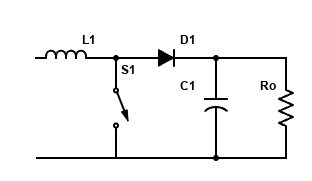
\includegraphics[width=0.8\textwidth]{img/Boost conv.png}
\end{center}

\section{Steady state, lossless}

\noindent
Dalla condizione in steady state deriva che la media della tensione sull'induttore e della corrente nel condensatore durante un periodo di switch è nulla, quindi

\vspace{0.5em}
\begin{align*}
    \langle v_L \rangle_{T_{\mathrm{sw}}} &= (1 - \delta)\,(V_{in} - V_{out}) + \delta\,V_{in} = V_{in} - (1 - \delta)\,V_{out} = 0\,V \implies V_{out} = \frac{V_{in}}{1 - \delta} \\[1em]
    %
    \langle i_c \rangle_{T_{\mathrm{sw}}} &= (1 - \delta)\,\langle i_L - i_{out} \rangle_{T_{\mathrm{sw}}} - \delta\,\langle i_{out} \rangle_{T_{\mathrm{sw}}} = 0\,A \implies I_{out} = I_{in}\, (1 - \delta) \\[1em]
    %
    \langle i_{in} \rangle_{T_{\mathrm{sw}}} &= \langle i_L \rangle_{T_{\mathrm{sw}}} \implies I_{out} = I_{in}\,(1 - \delta) = I_L\,(1 - \delta)
\end{align*}
\vspace{0.5em}

\noindent
Da qui si può ricavare il valore del duty cycle per avere il corretto rapporto tra tensione in ingresso e tensione in uscita

\vspace{0.5em}
\begin{align*}
    V_{out} = \frac{V_{in}}{1 - \delta} 
    \implies 1 - \delta = \frac{V_{in}}{V_{out}} \simeq 0.275 
    \implies \delta \simeq 0.725
\end{align*}
\vspace{0.5em}

\begin{center}
    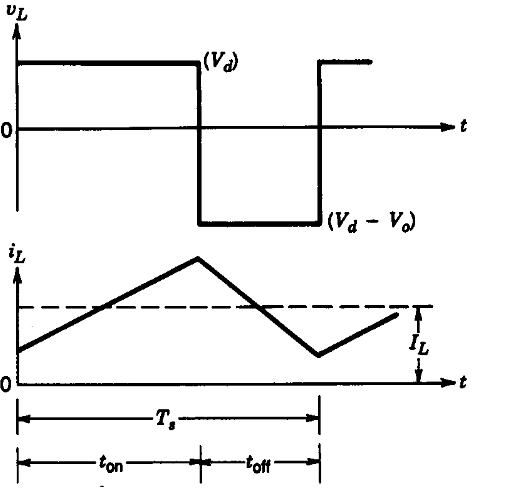
\includegraphics[width=0.8\textwidth]{img/Boost CCM graph.png}
\end{center}

\noindent
Durante il \(t_{on}\) la \(i_L \simeq \frac {V_{in}}{L} \cdot t \), durante il \(t_{off}\) invece \(i_L \simeq \frac {V_{in} - V_{out}}{L} \cdot t \).
Per rispettare la specifica di funzionamento \(CCM\) faccio in maniera tale che il \( \frac{\Delta i_L}{2} \) sia sempre minore di \(I_L \), quindi considero il più basso valore assumibile da \(I_L\) e impongo la condizione

\vspace{0.5em}
\begin{align*}
    \frac{\Delta i_L}{2} < {I_{Lmin}}
\end{align*}
\vspace{0.5em}

\noindent
il valore di \(I_{Lmin}\) si ha in corrispondenza di \(R_{omax}\) e \(V_{outmin}\)

\vspace{0.5em}
\[
    I_{L_{\min}} = I_{out_{\min}} \cdot \frac{1}{1 - \delta} = \frac{V_{out} - r}{R_{o_{\max}}} \cdot \frac{1}{1 - \delta} \simeq \frac{11.988\,V}{1000\,\Omega} \cdot 3.\overline{63} \simeq 43.593\,mA
\]
\vspace{0.5em}

\noindent
da qui posso ricavare la condizione di massima \( \Delta i_L \) con la quale dimensiono L

\vspace{0.5em}
\[
    \Delta i_L = \frac{V_{in}}{L} \cdot \delta T_{\mathrm{sw}} < 2 \cdot {I_{L_{\min}}} \implies L > \frac{V_{in}}{2I_{L_{\min}}} \cdot \frac {\delta}{f_{\mathrm{sw}}} \simeq 45.73 \mu H
\]
\vspace{0.5em}

\noindent
per l'induttore è stato scelto il RFS1317-334KL: un induttore da \(330 \mu H\) con DCR di \(286 m \Omega\). \\
Con un induttore di queste dimensioni il funzionamento in CCM è garantito fino ad un carico di 
\[
R_{out} \simeq \frac{V_{out}}{V_{in}} \frac{Lf_{sw}}{\delta(1-\delta)} \simeq 7.2k\Omega 
\]


\vspace{0.5em}
\noindent
Link al datasheet dell'induttore scelto 
\begin{center}
    \url{https://www.coilcraft.com/en-us/products/power/shielded-inductors/high-current-radial-lead/rfs/rfs1317/?skuId=6023}
\end{center}
\vspace{0.5em}

\noindent
Adesso dimensioniamo anche il condensatore cercando di rispettare la specifica sul ripple della \(V_{out}\) 

\vspace{0.5em}
\[
    \Delta V_{out} \simeq \frac{I_{out}}{C} \delta T_{sw} = \frac{V_{out}}{R_o C} \delta T_{sw} 
    \implies \frac{\Delta V_{out}}{V_{out}} < \frac{r}{V_{out}} = 0.001 
    \implies C > \frac{V_{out}}{r} \cdot \frac{\delta T_{sw}}{R_o}
\]
\vspace{0.5em}

\noindent
Anche qui considero il caso peggiore (ripple maggiore), ovvero quello con \(R_o\) minima

\vspace{0.5em}
\[
    C > \frac{V_{out}}{r} \cdot \frac{\delta T_\mathrm{sw}}{R_{o_{\min}}} \simeq 12.083 \mu F
\]
\vspace{0.5em}


\noindent
per il condensatore è stato scelto il 100SXE18H: un condensatore elettrolitico da \(18 \mu F\) con tolleranza del \(20 \%\ \), una tensione massima di \(100 V_{DC}\) e una resistenza serie equivalente di \(30 m \Omega \).

\vspace{0.5em}
\noindent
Link al datasheet del condensatore scelto 
\begin{center}
    \url{https://www.mouser.it/ProductDetail/Panasonic/100SXE18M%2b3?qs=sGAEpiMZZMvwFf0viD3Y3bXvgfG2gej7S5yOo2TLmT88R8WFNeVXkA%3D%3D}
\end{center}
\vspace{0.5em}

\noindent
I dati sono stati verificati con LTSpice utilizzando il circuito \autoref{fig:LTSpice circuito}

\begin{figure}[h]
    \centering
    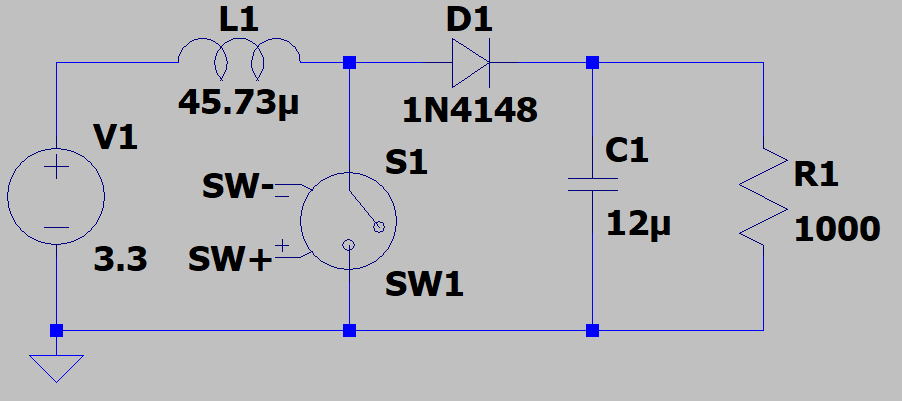
\includegraphics[width=1\textwidth]{img/Boost conv LTSpice.png}
    \caption{Circuito per la simulazione steady state, lossless}
    \label{fig:LTSpice circuito}
\end{figure}

\newpage

\noindent
Prima è stata fatta la simulazione utilizzando \(R_o = 1000 \Omega\) e leggendo la corrente nell'induttore \autoref{fig:grafico delta i_L}

\begin{figure}[h]
    \centering
    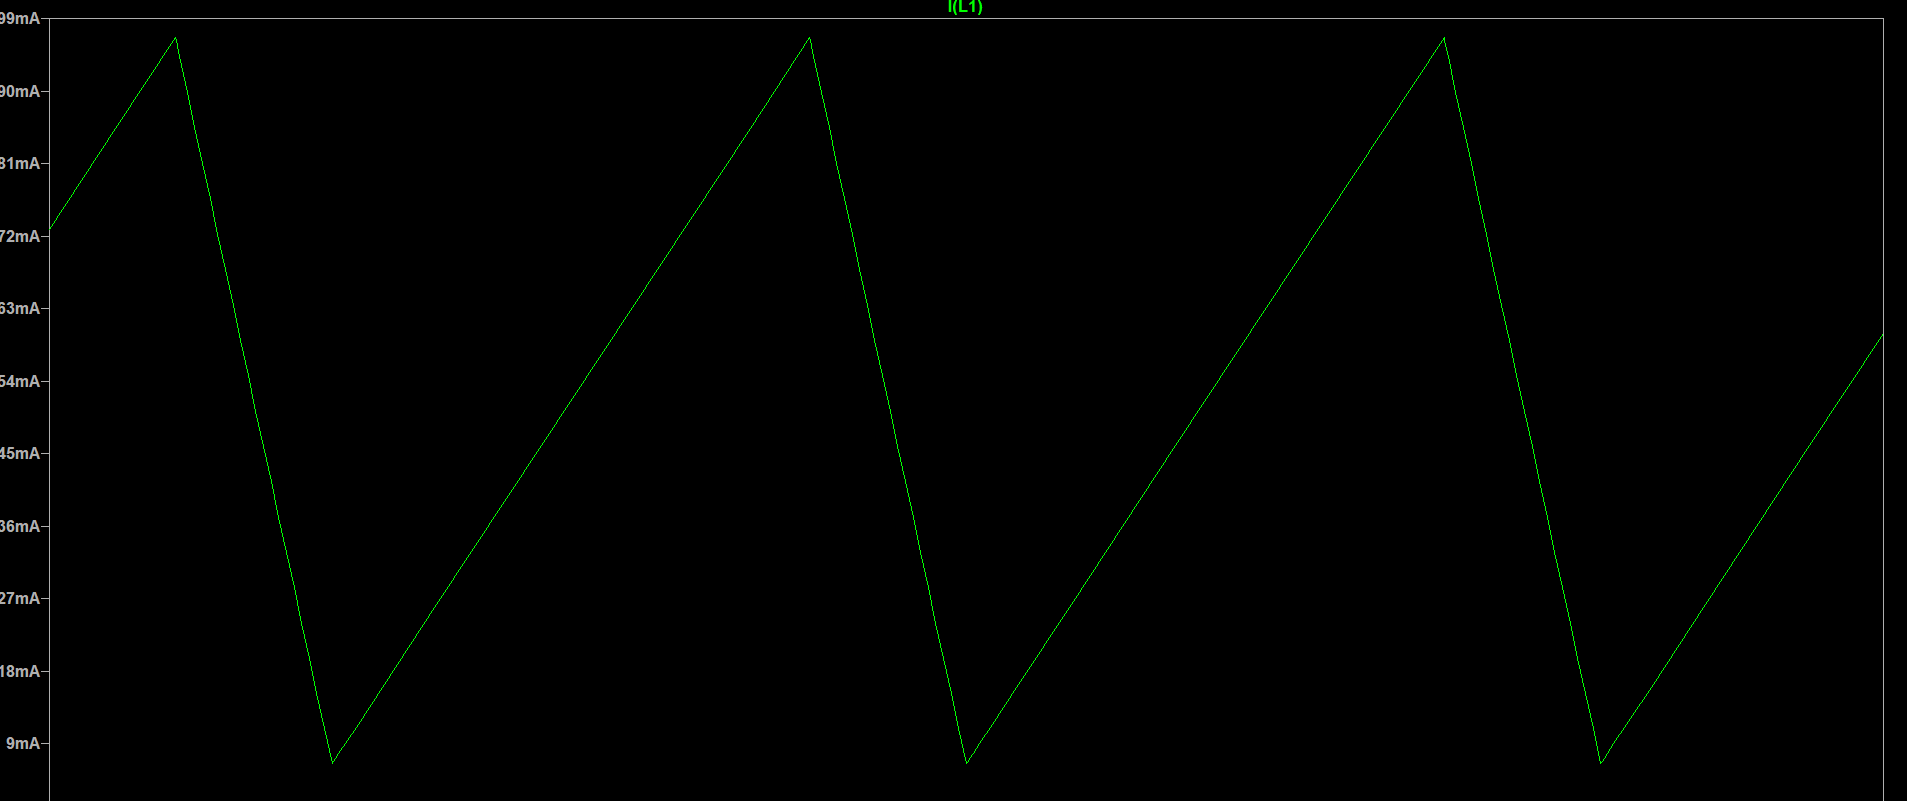
\includegraphics[width=1\textwidth]{img/grafico delta i_L.png}
    \caption{Simulazione corrente nell'induttore a regime}
    \label{fig:grafico delta i_L}
\end{figure}

\noindent
Dalla simulazione \autoref{fig:grafico delta i_L}, risulta che (l'onda blu è il segnale PWM, mentre l'onda verde è la corrente nell'induttore) il \(\Delta i_L \simeq 87.2 mA\) che è all'incirca \(2 \cdot I_L \) come calcolato in precedenza.

\vspace{0.5em}
\noindent
Poi è stata fatta la simulazione utilizzando \(R_o = 100 \Omega\) e leggendo la tensione in uscita \autoref{fig:grafico delta V_out}

\begin{figure}[h]
    \centering
    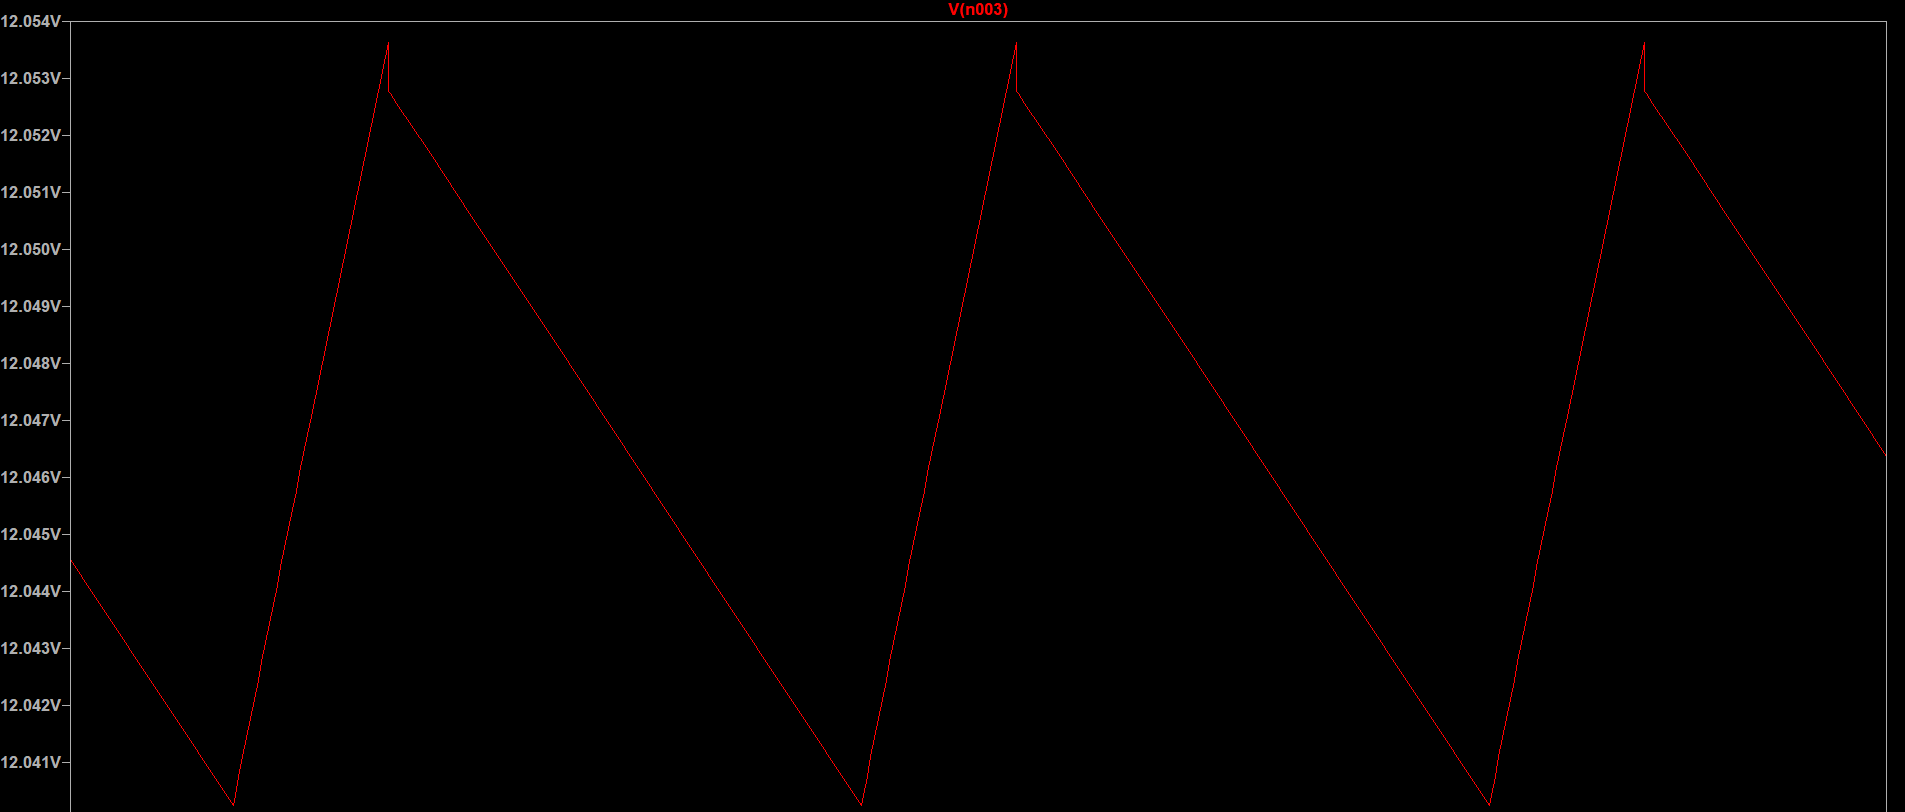
\includegraphics[width=1\textwidth]{img/grafico delta V_out.png}
    \caption{Simulazione tensione di uscita a regime}
    \label{fig:grafico delta V_out}
\end{figure}

\noindent
Dalla simulazione \autoref{fig:grafico delta V_out}, risulta che (l'onda è la tensione di uscita dal convertitore) il \(\Delta V_{out} \simeq 0.013V\) e considerando che \(r < 0.001 \cdot V_{out} = 0.012V\) anche qui il risultato è concorde con i calcoli.

\noindent
Per mantenere del margine con i dati teorici, per il condensatore e l'induttore sono stati scelti dei valori maggiori rispetto ai minimi calcolati, in modo da contrastare il derating dei componenti e compensare gli effetti dei parametri parassiti. 

\newpage

\section{Steady state, con perdite}

Per l'analisi delle perdite devo introdurre tutti i componenti dissipativi del circuito ideale come mostrato in \autoref{fig:Boost conv losses}

\begin{figure}[h]
    \centering
    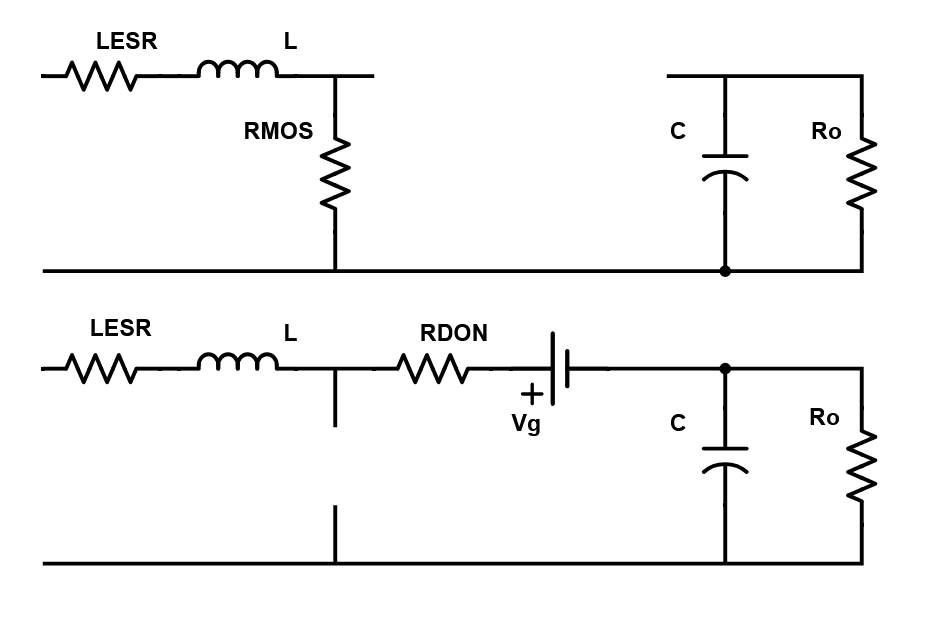
\includegraphics[width=1\textwidth]{img/Boost conv losses.png}
    \caption{Boost converter con perdite}
    \label{fig:Boost conv losses}
\end{figure}

\noindent
applicando le stesse formule di prima, siamo in grado di ricavare il \(VCR = \frac{V_{out}}{V_{in}}\) con perdite e il rendimento \(\eta\).

\vspace{0.5em}
\begin{align*}
    \langle v_L \rangle_{T_{\mathrm{sw}}} &= (1 - \delta)\,\left[ V_{in} - R_{LESR} \cdot I_L - (V_{out} + V_{\gamma} + R_{Don} \cdot I_L ) \right] + \delta\,\left[V_{in} - (R_{LESR} + R_{MOS} ) \cdot I_L\right] \\ &= 0V \\[1em]
    %
    \langle i_c \rangle_{T_{\mathrm{sw}}} &= (1 - \delta)\,\langle i_L - i_{out} \rangle_{T_{\mathrm{sw}}} - \delta\,\langle i_{out} \rangle_{T_{\mathrm{sw}}} = 0\,A \implies I_{out} = I_{in}\, (1 - \delta) \\[1em]
    %
    \langle i_{in} \rangle_{T_{\mathrm{sw}}} &= \langle i_L \rangle_{T_{\mathrm{sw}}} \implies I_{out} = I_{in}\,(1 - \delta) = I_L\,(1 - \delta)
\end{align*}
\vspace{0.5em}

\noindent
Da cui si può ricavare la relazione ingresso uscita del convertitore

\vspace{0.5em}
\begin{align*}
    V_{out} = \frac{V_{in}}{1-\delta} - V_{\gamma} - \left[ \frac{ \delta }{1-\delta} R_{MOS} + \frac{1}{1-\delta}R_{LESR} + R_{Don}\right] \cdot \frac{I_{out}}{1-\delta} = \frac{V_{in}}{1-\delta} - V_{\gamma} - R_{eq} I_{out}
\end{align*}
\vspace{0.5em}

\noindent
da queste formule si può arrivare al modello semplificato del Boost converter con perdite che è il circuito mostrato in \autoref{fig:eq circ losses}

\newpage
\vspace{0.5em}
\begin{figure}[h]
    \centering
    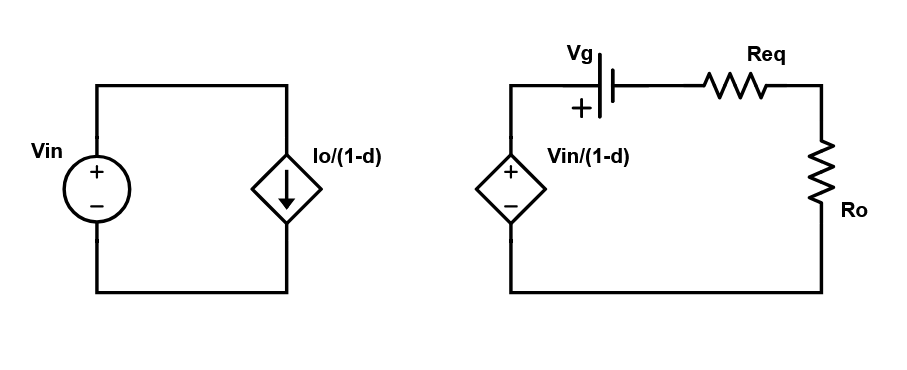
\includegraphics[width=1\textwidth]{img/Eq circ losses.png}
    \caption{Circuito equivalente con perdite}
    \label{fig:eq circ losses}
\end{figure}
\vspace{0.5em}

\noindent
da cui si ricava il \(VCR\) con perdite e il rendimento

\vspace{0.5em}
\[
\begin{cases}
   \begin{aligned}
       VCR &= \frac{V_{out}}{V_{in}} = \frac{1}{V_{in}} \cdot \left[ \frac{V_{in}}{1-\delta} - V_{\gamma} \right] \cdot \frac{R_o}{R_o + R_{eq}} \\ &= \frac{1}{1-\delta} \cdot \frac{1-\frac{V_{\gamma}}{V_{in}} (1 - \delta)}{1+\frac{\delta}{(1-\delta)^2}\frac{R_{MOS}}{R_o} + \frac{R_{LESR}}{(1-\delta)^2} \frac{1}{R_o} + \frac{R_{Don}}{R_o \cdot (1-\delta)}}
   \end{aligned}
       \\[2em]
    \begin{aligned}
       \frac{I_{out}}{I_{in}} = \frac{I_{out}}{I_{L}} = 1 - \delta
    \end{aligned}
\end{cases}
\]
\vspace{0.5em}

\noindent
il rendimento si calcola come

\begin{align*}
    \eta = \frac{P_{out}}{P_{in}} = \frac{V_{out}I_{out}}{V_{in}I_{in}} = VCR \frac{I_{out}}{I_{in}} 
    = \frac{1-\frac{V_{\gamma}}{V_{in}} (1 - \delta)}{1+\frac{\delta}{(1-\delta)^2}\frac{R_{MOS}}{R_o} + \frac{R_{LESR}}{(1-\delta)^2} \frac{1}{R_o} + \frac{R_{Don}}{R_o \cdot (1-\delta)}}
\end{align*}

\vspace{0.5em}
\begin{figure}[h]
    \centering
    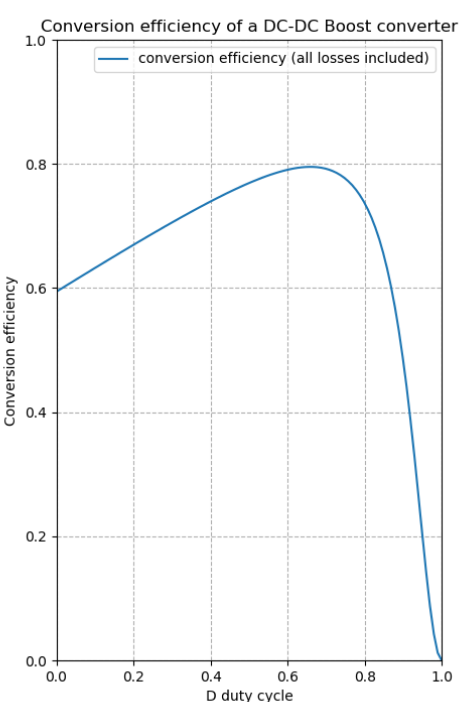
\includegraphics[width=0.33\textwidth]{img/conv_coeff.png}
    \caption{Grafico rendimento al variare del duty cycle}
    \label{fig:conv_coeff}
\end{figure}
\vspace{0.5em}

\newpage
\noindent
Si nota come ci sia una parte del rendimento, dominata dalle perdite per conduzione, dove la \(P_{loss} \ \alpha \ I_{out} ^ 2\) e \(P_{out} \ \alpha \ I_{out}\), che è la parte in cui il rendimento decresce all'aumentare del duty cycle e una parte dominata dalle perdite di switching, quelle dovute alle capacità parassite del MOS.
\noindent
Per la scelta del MOS e del diodo, considero le massime tensioni e correnti che devono sopportare e cerco le soluzioni con le capacità e le resistenze parassite più piccole.

\vspace{0.5em}
\begin{align*}
    V_{MAX_{MOS}} &= V_{out} = 12V \\
    V_{MAX_{diodo}} &= V_{out} - V_{in} = 8.7V \\
    I_{MAX_{MOS}} &= I_{L_{MAX}} + \Delta i_L = I_{out_{MAX}} + \Delta i_L \simeq 202 mA \\
    I_{MAX_{diodo}} &= I_{out_{MAX}} \simeq 120 mA
\end{align*}
\vspace{0.5em}

\noindent
Il transistor scelto è il IRFH7921: un N-MOS da \(34 A\) con una tensione \(V_{DS}\) massima di \(30 V\) e una resistenza drain source di \(8.5 m \Omega \).

\vspace{0.5em}
\noindent
Link al datasheet del transistor scelto 
\begin{center}
    \url{https://www.infineon.com/part/IRFH7921}
\end{center}
\vspace{0.5em}

\noindent
Il diodo scelto è il BAS3005A-02V: un diodo da \(500 mA\) con una tensione \(V_{\gamma}\) massima di \(500 m V\) e una resistenza serie di \(267 m \Omega \) ricavata dal grafico ( \(V_F\) , \(I_F\) ) presente nel datasheet.

\vspace{0.5em}
\noindent
Link al datasheet del diodo scelto 
\begin{center}
    \url{https://www.infineon.com/part/BAS3005A-02V}
\end{center}
\vspace{0.5em}

\noindent
Usando la formula del rendimento trovata sopra risulta che \( \eta \in [91 \%\ , 95 \%\ ] \).
La stima è stata fatta trascurando la resistenza serie del condensatore e trascurando le capacità del transistor e del diodo.
Calcoliamo le potenze dissipate per i vari componenti

\vspace{0.5em}
\noindent
Le perdite per switching sono:
\vspace{0.5em}
\begin{align*}
    P_{{MOS}_{switching}} &= f_{\mathrm{sw}} \cdot \left[ C_{gs} \Delta V_{gs}^2 + C_{gd} \Delta V_{gd}^2 + C_{ds} \Delta V_{ds}^2 \right] \simeq 33.1 mW
\end{align*}
\vspace{0.5em}

\noindent
Le perdite per conduzione sono:
\vspace{0.5em}
\begin{align*}
    P_{MOS} &= \delta R_{MOSon} \left(\frac{I_{out}}{1-\delta} \right)^2\\
    P_D &= (1-\delta) V_\gamma I_{out} + (1-\delta)R_{Don}I_{out}^2\\
    P_L &= R_{LESR} \left(\frac{I_{out}}{1-\delta} \right)^2 \\
    P_c &= \frac{r^2}{R_{CESR}}
\end{align*}
\vspace{0.5em}

\noindent
Così si arriva ad un rendimento effettivo compreso tra \(\eta \in [89.7 \%\ , 94.3 \%\ ] \) che essendo sempre maggiore del \(70 \%\) rispetta, almeno analiticamente, le specifiche, adesso procediamo alla verifica con il simulatore.

\newpage
\noindent
Analiticamente risulta che la potenza persa totale nei vari componenti sia distribuita secondo il grafico a torta in \autoref{fig:grafico_a_torta}

\vspace{0.5em}
\begin{figure}[h]
    \centering
    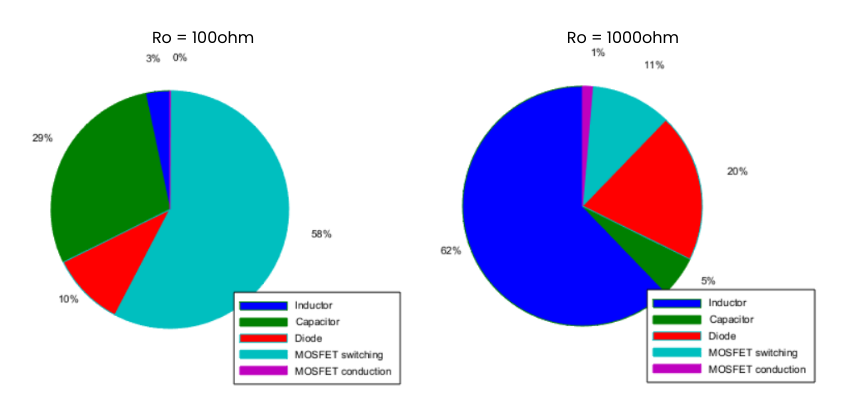
\includegraphics[width=0.8\textwidth]{img/pie energy graph.png}
    \caption{Grafico della percentuale di potenza dissipata nei vari componenti del circuito}
    \label{fig:grafico_a_torta}
\end{figure}
\vspace{0.5em}

Il circuito utilizzato per effettuare la simulazione è quello in \autoref{fig:circuito losses}

\vspace{0.5em}
\begin{figure}[h]
    \centering
    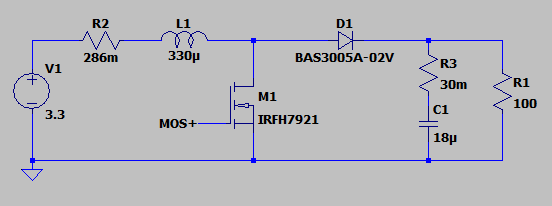
\includegraphics[width=1\textwidth]{img/Boost conv losses LTSpice.png}
    \caption{Circuito per il calcolo dell'efficienza}
    \label{fig:circuito losses}
\end{figure}
\vspace{0.5em}

\noindent
Durante la simulazione è stato calcolato il rendimento (calcolato come rapporto tra la potenza media dissipata sul carico diviso la potenza media erogata dal generatore) del circuito a regime per un carico di \(100 \Omega\) e per un carico di \(1000 \Omega\).
Con un carico di \(100 \Omega\) ho un rendimento del \( \eta \simeq 90.9 \% \), mentre con un carico di \(1000 \Omega\) ho un rendimento del \(\eta \simeq 87.5 \% \)


\newpage
\section{Modello dinamico}
Rimuovendo l'ipotesi di steady state, le forme d'onda possono variare da un periodo di switching all'altro, quindi si analizzano due termini:

\begin{itemize}
    \item \textbf{Valor medio del segnale}, ipotizzato costante per ogni periodo di switch
    \item \textbf{Termini del prim'ordine}, ovvero variazioni delle grandezze in gioco all'interno di un periodo di switching
\end{itemize}

\noindent
Le grandezze di controllo vengono rappresentate quindi come somma di \(X\) (valor medio) e \( \tilde{x}\) (contributo del prim'ordine) 

\vspace{0.5em}
\begin{align*}
    <x> &= X + \tilde{x} \\
    <x><y> &= (X + \tilde{x})(Y + \tilde{y}) = XY + X\tilde{y} + Y \tilde{x} + \tilde{x}\tilde{y} \simeq XY + ( X\tilde{y} + Y \tilde{x} )
\end{align*}
\vspace{0.5em}

\noindent
Riprendiamo adesso il circuito \autoref{fig:Boost conv losses} e applichiamo stavolta le relazioni costitutive dell'induttore e del condensatore

\vspace{0.5em}
\[
\begin{cases}
    \begin{aligned}
       <v_L> = L \frac{d}{dt}<i_L>
    \end{aligned}
       \\[2em]
    \begin{aligned}
       <i_c> = L \frac{d}{dt}<v_c>
    \end{aligned}
       \\[2em]
    \begin{aligned}
       <i_{in}> = <i_L>
    \end{aligned}
\end{cases}
\]
\vspace{0.5em}

\noindent
Riscrivendo le grandezze in gioco come somma dei contributi di ordine inferiore al secondo si ottiene:

\begin{itemize}
    \item \(<v_L> = V_L + \tilde{v_L}\)
    \item \(<i_c> = I_c + \tilde{i_c}\)
    \item \(\delta = D + \tilde{\delta}\)
\end{itemize}

\vspace{0.5em}
\begin{align*}
    <v_L> &= \delta <v_{in}> + (1-\delta)(<v_{in}>-<v_{out}>) \implies \\
    V_L + \tilde{v_L} &\simeq V_{in} - (1-D)V_{out} + \tilde{\delta}V_{out}+\tilde{v_{in}} - (1-D)\tilde{v_{out}} = L \frac{d}{dt}\tilde{i_L}
    \\[2em]
    <i_c> &= -\delta <i_{out}> + (1-\delta)(<i_{L}>-<i_{out}>) \implies \\
    I_c + \tilde{i_c} &\simeq -I_{out} + (1-D)I_{L} - \tilde{\delta}I_{L} -\tilde{i_{out}} + (1-D)\tilde{i_{L}} = C \frac{d}{dt}\tilde{v_{out}}
    \\[2em]
    <i_L> &= <i_{in}>
\end{align*}
\vspace{0.5em}

\newpage
\noindent
Da qui, separando i termini di ordine 0 dai termini di ordine 1, ottengo sia le relazioni trovate con il modello steady state lossless, sia le relazioni utili per progettare il sistema di controllo.

\vspace{0.5em}
\[
\begin{cases}
    \begin{aligned}
       V_{in} - (1-D)V_{out} = L\frac{d}{dt}V_L = 0V \xleftarrow{} V_L ~ \grave{e} ~ una ~ grandezza ~ costante ~ nel ~ periodo ~ T_{\mathrm{sw}}
    \end{aligned}
       \\[2em]
    \begin{aligned}
       \tilde{\delta}V_{out} + \tilde{v_{in}} - (1-D)\tilde{v_{out}} = L\frac{d}{dt}\tilde{v_L}
    \end{aligned}
\end{cases}
\]
\[
\begin{cases}
    \begin{aligned}
       -I_{out} + (1-D)I_{L} = C\frac{d}{dt}V_c = 0A \xleftarrow{} I_c ~ \grave{e} ~ una ~ grandezza ~ costante ~ nel ~ periodo ~ T_{\mathrm{sw}}
    \end{aligned}
       \\[2em]
    \begin{aligned}
       -\tilde{\delta}I_{L} - \tilde{i_{out}} + (1-D)\tilde{i_{L}} = C\frac{d}{dt}\tilde{v_c}
    \end{aligned}
\end{cases}
\]
\[
\begin{cases}
    \begin{aligned}
       I_L = I_{in}
    \end{aligned}
       \\[2em]
    \begin{aligned}
       \tilde{i_L} = \tilde{i_{in}}
    \end{aligned}
\end{cases}
\]
\vspace{0.5em}

\noindent
Adesso possiamo disegnare il modello circuitale lineare tempo invariante che descrive le variazioni delle grandezze in gioco in un periodo di switching \autoref{fig:circuito LTI variazioni}

\vspace{0.5em}
\begin{figure}[h]
    \centering
    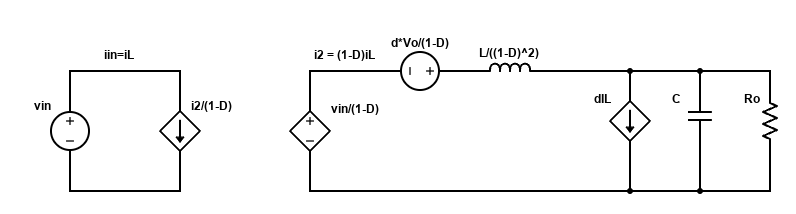
\includegraphics[width=1\textwidth]{img/circuito LTI variazioni.png}
    \caption{Modello LTI delle grandezze al prim'ordine}
    \label{fig:circuito LTI variazioni}
\end{figure}
\vspace{0.5em}

\noindent
portando il modello trovato in forma canonica, quindi con il modello del trasformatore in continua, tutti i generatori a sinistra del trasformatore e tutti i componenti passivi a destra si ottiene \autoref{fig:circuito LTI transf_DC}

\newpage
\vspace{0.5em}
\begin{figure}[h]
    \centering
    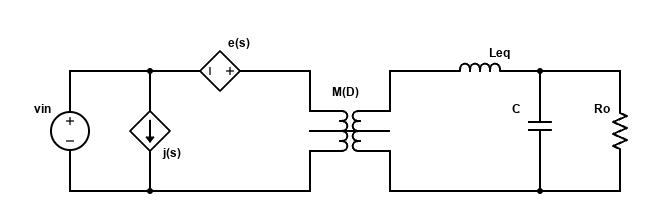
\includegraphics[width=1\textwidth]{img/circuito LTI con transf_DC.png}
    \caption{Modello LTI delle grandezze al prim'ordine}
    \label{fig:circuito LTI transf_DC}
\end{figure}
\vspace{0.5em}

\vspace{0.5em}
\[
\begin{cases}
    \begin{aligned}
       e(s) = \tilde{\delta}V_{out} - \tilde{\delta}I_L \frac{sL}{1-D}
    \end{aligned}
       \\[2em]
    \begin{aligned}
       j(s) = \frac{\tilde{\delta}}{1-D} I_L
    \end{aligned}
        \\[2em]
    \begin{aligned}
        L_{eq} = \frac{L}{(1-D)^2}
    \end{aligned}
        \\[2em]
    \begin{aligned}
        M(D) = \frac{1}{1-D}
    \end{aligned}
    
\end{cases}
\]
\vspace{0.5em}

\noindent
Definisco adesso la funzione di trasferimento del filtro passa basso in uscita dal trasformatore in continua \autoref{fig:LPF(s)}

\vspace{0.5em}
\begin{figure}[h]
    \centering
    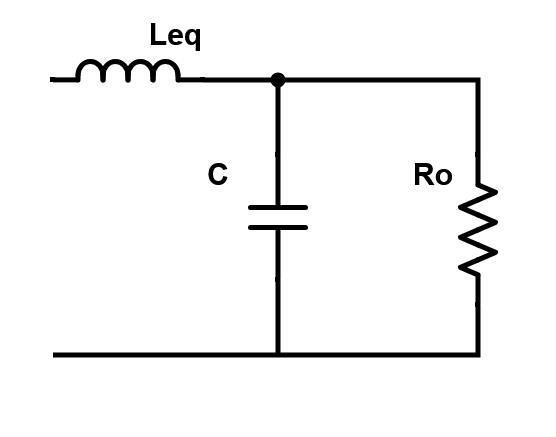
\includegraphics[width=0.35\textwidth]{img/LPF(s).png}
    \caption{Circuito di filtro in uscita}
    \label{fig:LPF(s)}
\end{figure}
\vspace{0.5em}

\vspace{0.5em}
\[
    H_{LPF}(s) = \frac{\frac{R}{1+sRC}}{\frac{R}{1+sRC} + sL_{eq}} = \frac{1}{ (\frac{1}{R} + sC)sL_{eq} + 1 } = \frac{(1-D)^2}{(\frac{1}{R} + sC)sL + (1 -D)^2}
\]
\vspace{0.5em}

\newpage
\noindent
Posso trovare adesso i vari guadagni necessari a costruire lo schema a blocchi del sistema ad anello aperto da controllare.

\vspace{0.5em}
\begin{align*}
    G_{vd} &= \left. \frac{\tilde{v_{out}}}{\tilde{\delta}} \right|_{\substack{ \tilde{i_{out}} = 0A \\ \tilde{v_{in}} = 0V }} = \frac{e(s)}{\tilde{\delta}} M(D) H_{LPF}(s) \\
    G_{vg} &= \left. \frac{\tilde{v_{out}}}{\tilde{v_{in}}} \right|_{\substack{ \tilde{i_{out}} = 0A \\ \tilde{\delta} = 0 }} = M(D) H_{LPF}(s) \\
    Z_{out} &= \left. \frac{\tilde{v_{out}}}{i_{out}} \right|_{\substack{ \tilde{\delta} = 0 \\ \tilde{v_{in}} = 0V }} = sL_{eq} //\frac{1}{sC}//R = \frac{sL}{(1-D)^2} H_{LPF}(s)
\end{align*}
\vspace{0.5em}

\newpage
\noindent
Lavorando sulle funzioni di trasferimento calcolate si possono portare in forma canonica

\vspace{0.5em}
\begin{align*}
    G_{vd} &= \frac{V_{out}}{1-D} \frac{1-s\frac{LI_L}{V_{out}(1-D)}}{1+s\frac{L}{R(1-D)^2} +s^2 \frac{LC}{(1-D)^2}} = K \frac{1-s\frac{1}{\omega_z}}{1+\frac{s}{Q \omega_o} + \frac{s^2}{\omega_o^2}}
\end{align*}
\vspace{0.5em}

\vspace{0.5em}
\[
\begin{cases}
    \begin{aligned}
       K = \frac{V_{out}}{1-D} \simeq 43.63 V
    \end{aligned}
       \\[2em]
    \begin{aligned}
       \omega_z = \frac{V_{out}(1-D)}{LI_L} = \frac{V_{out}(1-D)}{L}\frac{1-D}{I_{out}} \simeq 
        \begin{cases}
            22916.67 \frac{rad}{s} \xleftarrow{} R = 100 \Omega\\
            229166.67 \frac{rad}{s} \xleftarrow{} R = 1000 \Omega
        \end{cases}
    \end{aligned}
       \\[2em]
    \begin{aligned}
       \omega_o = \frac{1-D}{\sqrt{LC}} \simeq 3568.12 \frac{rad}{s}
    \end{aligned}
       \\[2em]
    \begin{aligned}
       Q = \frac{R}{L} \frac{(1-D)^2}{\omega_o} = R \sqrt{\frac{C}{L}} (1-D) \simeq 
        \begin{cases}
            6.423 \frac{rad}{s} \xleftarrow{} R = 100 \Omega \\
            64.226 \frac{rad}{s} \xleftarrow{} R = 1000 \Omega
        \end{cases}
    \end{aligned}  
\end{cases}
\]
\vspace{0.5em}

\vspace{0.5em}
\begin{align*}
    G_{vg} &= \frac{1}{1-D} \frac{1}{1 + s \frac{L}{R}\frac{1}{(1-D)^2} + s^2 \frac{LC}{(1-D)^2}} = K \frac{1}{1+\frac{s}{Q \omega_o} + \frac{s^2}{\omega_o^2}}
\end{align*}
\vspace{0.5em}

\vspace{0.5em}
\[
\begin{cases}
    \begin{aligned}
       K = \frac{1}{1-D} \simeq 3.63
    \end{aligned}
       \\[2em]
    \begin{aligned}
       \omega_o = \frac{1-D}{\sqrt{LC}} \simeq 3568.12 \frac{rad}{s}
    \end{aligned}
       \\[2em]
    \begin{aligned}
       Q = \frac{R(1-D)^2}{L} \frac{1}{\omega_o} = R \sqrt{\frac{C}{L}}(1-D) \simeq 
        \begin{cases}
            6.423 \frac{rad}{s} \xleftarrow{} R = 100 \Omega \\
            64.226 \frac{rad}{s} \xleftarrow{} R = 1000 \Omega
        \end{cases}
    \end{aligned}
\end{cases}
\]
\vspace{0.5em}

\vspace{0.5em}
\begin{align*}
    Z_{out} &= \frac{L}{(1-D)^2}\frac{s}{1 + s \frac{L}{R}\frac{1}{(1-D)^2} + s^2 \frac{LC}{(1-D)^2}} = K \frac{s}{1+\frac{s}{Q \omega_o} + \frac{s^2}{\omega_o^2}}
\end{align*}
\vspace{0.5em}

\vspace{0.5em}
\[
\begin{cases}
    \begin{aligned}
       K = \frac{L}{(1-D)^2} \simeq 4.36 \cdot 10^{-3} H
    \end{aligned}
       \\[2em]
    \begin{aligned}
       \omega_o = \frac{1-D}{\sqrt{LC}} \simeq 3568.12 \frac{rad}{s}
    \end{aligned}
       \\[2em]
    \begin{aligned}
       Q = \frac{R(1-D)^2}{L} \frac{1}{\omega_o} = R \sqrt{\frac{C}{L}}(1-D) \simeq 
        \begin{cases}
            6.423 \frac{rad}{s} \xleftarrow{} R = 100 \Omega \\
            64.226 \frac{rad}{s} \xleftarrow{} R = 1000 \Omega
        \end{cases}
    \end{aligned}
\end{cases}
\]
\vspace{0.5em}

\newpage
\noindent
\section{Progettazione del feedback}
Partendo dalle funzioni di trasferimento calcolate prima, posso disegnare lo schema a blocchi del sistema da controllare e del sistema retroazionato per il controllo

\vspace{0.5em}
\begin{figure}[h]
    \centering
    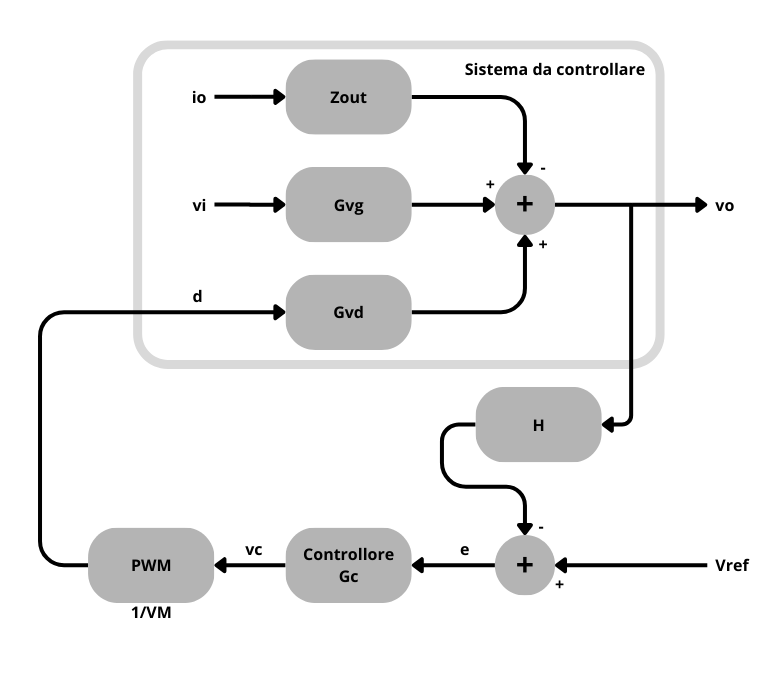
\includegraphics[width=1\textwidth]{img/Schema a blocchi boost DCDC.png}
    \caption{Schema a blocchi boost converter con feedback}
    \label{fig:schema a blocchi boost DCDC}
\end{figure}
\vspace{0.5em}

\noindent
Scrivo la funzione di trasferimento della tensione in uscita ad anello chiuso

\vspace{0.5em}
\[
\begin{cases}
    \begin{aligned}
       \tilde{v_{out}} = \tilde{\delta}G_{vd}(s)+\tilde{v_{in}}G_{vg}(s)-\tilde{i_{out}}Z_{out}(s)
    \end{aligned}
       \\[2em]
    \begin{aligned}
       \tilde{\epsilon} = \tilde{v_{out}}H(s) - \tilde{v_{ref}}
    \end{aligned}
       \\[2em]
    \begin{aligned}
       \tilde{\delta} = \frac{G_c(s)}{V_M} \tilde{\epsilon} = \frac{G_c(s)}{V_M}(\tilde{v_{out}H(s)-\tilde{v_{ref}}})
    \end{aligned}
\end{cases}
\]
\vspace{0.5em}

\[
    \tilde{v_{out}} = \frac{G_c(s)G_{vd}(s)}{V_M}(\tilde{v_{ref}}-\tilde{v_{out}}H(s)) + \tilde{v_{in}}G_{vg}(s)-\tilde{i_{out}}Z_{out}(s)
\]

\newpage
\vspace{0.5em}
\[
\begin{cases}
    \begin{aligned}
       T(s) = \frac{G_c(s)G_{vd}(s)}{V_M} H(s)
    \end{aligned}
       \\[2em]
    \begin{aligned}
       \tilde{v_{out}} = \frac{T(s)}{1+T(s)} \frac{\tilde{v_{ref}}}{H(s)} + \tilde{v_{in}} \frac{G_{vg}(s)}{1+T(s)} - \tilde{i_{out}}\frac{Z_{out}(s)}{1+T(s)}
    \end{aligned}
\end{cases}
\]
\vspace{0.5em}

\noindent
Le funzioni di trasferimento ad anello chiuso sono quindi

\vspace{0.5em}
\[
\begin{cases}
    \begin{aligned}
       G_{vg_{CL}}(s) = \frac{G_{vg}(s)}{1+T(s)}
    \end{aligned}
       \\[2em]
    \begin{aligned}
       Z_{out_{CL}}(s) = \frac{Z_{out}(s)}{1+T(s)}
    \end{aligned}
\end{cases}
\]
\vspace{0.5em}
\[
    \tilde{v_{out}} = \frac{T(s)}{1+T(s)} \frac{\tilde{v_{ref}}}{H(s)} + \tilde{v_{in}} G_{vg_{CL}}(s) - \tilde{i_{out}}{Z_{out_{CL}}(s)}
\]
\vspace{0.5em}

\vspace{0.5em}
\begin{figure}[h]
    \centering
    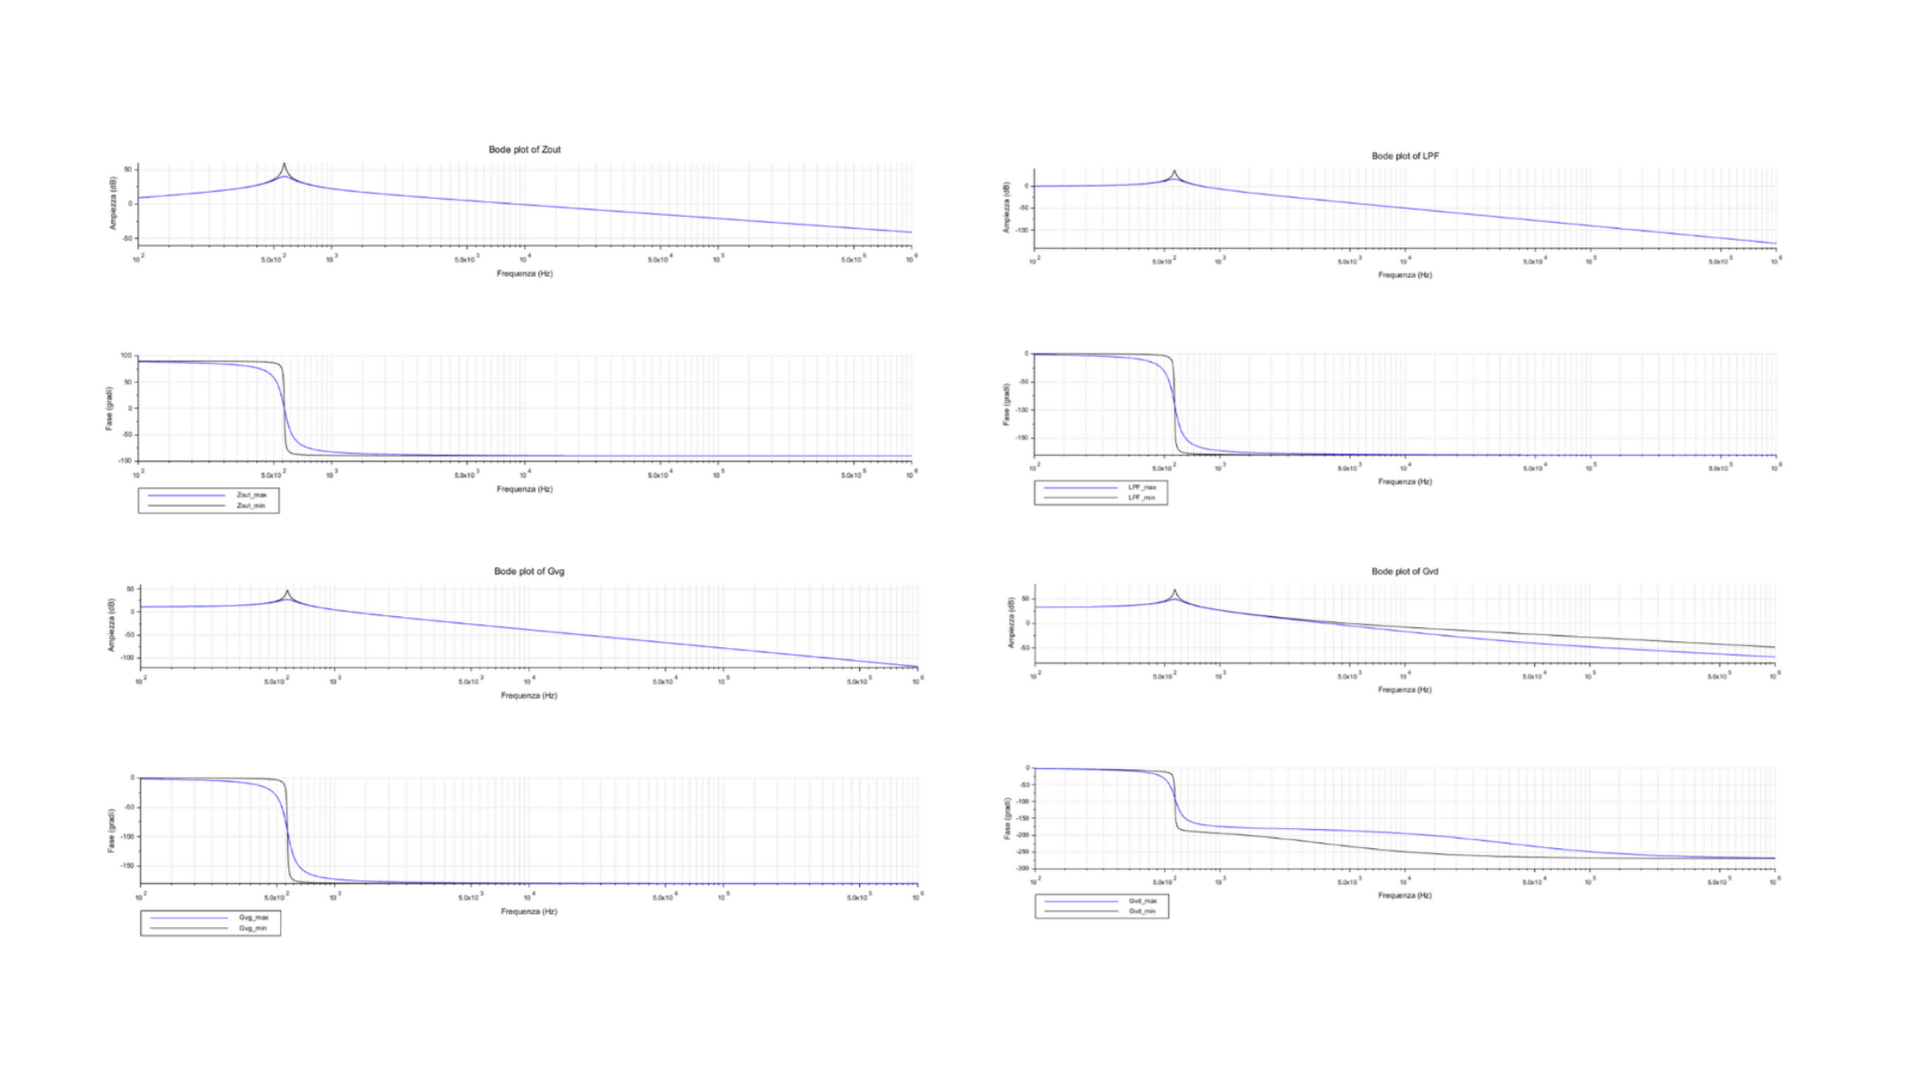
\includegraphics[width=1\textwidth]{img/bode diagrams OL.png}
    \caption{Diagrammi di bode delle funzioni di trasferimento calcolate, ad anello aperto}
    \label{fig:bode diagrams OL}
\end{figure}
\vspace{0.5em}

\newpage
\noindent
La funzione di trasferimento su cui dobbiamo lavorare per garantire la stabilità del sistema è la \(T(s)\) che possiamo scrivere come \(T_u(s)G_c(s)\) dove \(T_u(s)\) è la funzione di trasferimento, del sistema ad anello chiuso, che lega la tensione di uscita con il duty cycle del segnale PWM di controllo dell'interruttore.
Per la progettazione del controllore partiamo graficando la funzione di trasferimento di \(T_u(s)\), ovvero

\vspace{0.5em}
\begin{align*}
    T_u(s) = \frac{G_{vd}(s)}{V_M}H(s)
\end{align*}
\vspace{0.5em}

\noindent
con \(V_M = 1V\), ricavato dalle specifiche, e \(H(s) = \frac{V_{ref}}{V_{out}} = 0.275\) 

\vspace{0.5em}
\begin{figure}[h]
    \centering
    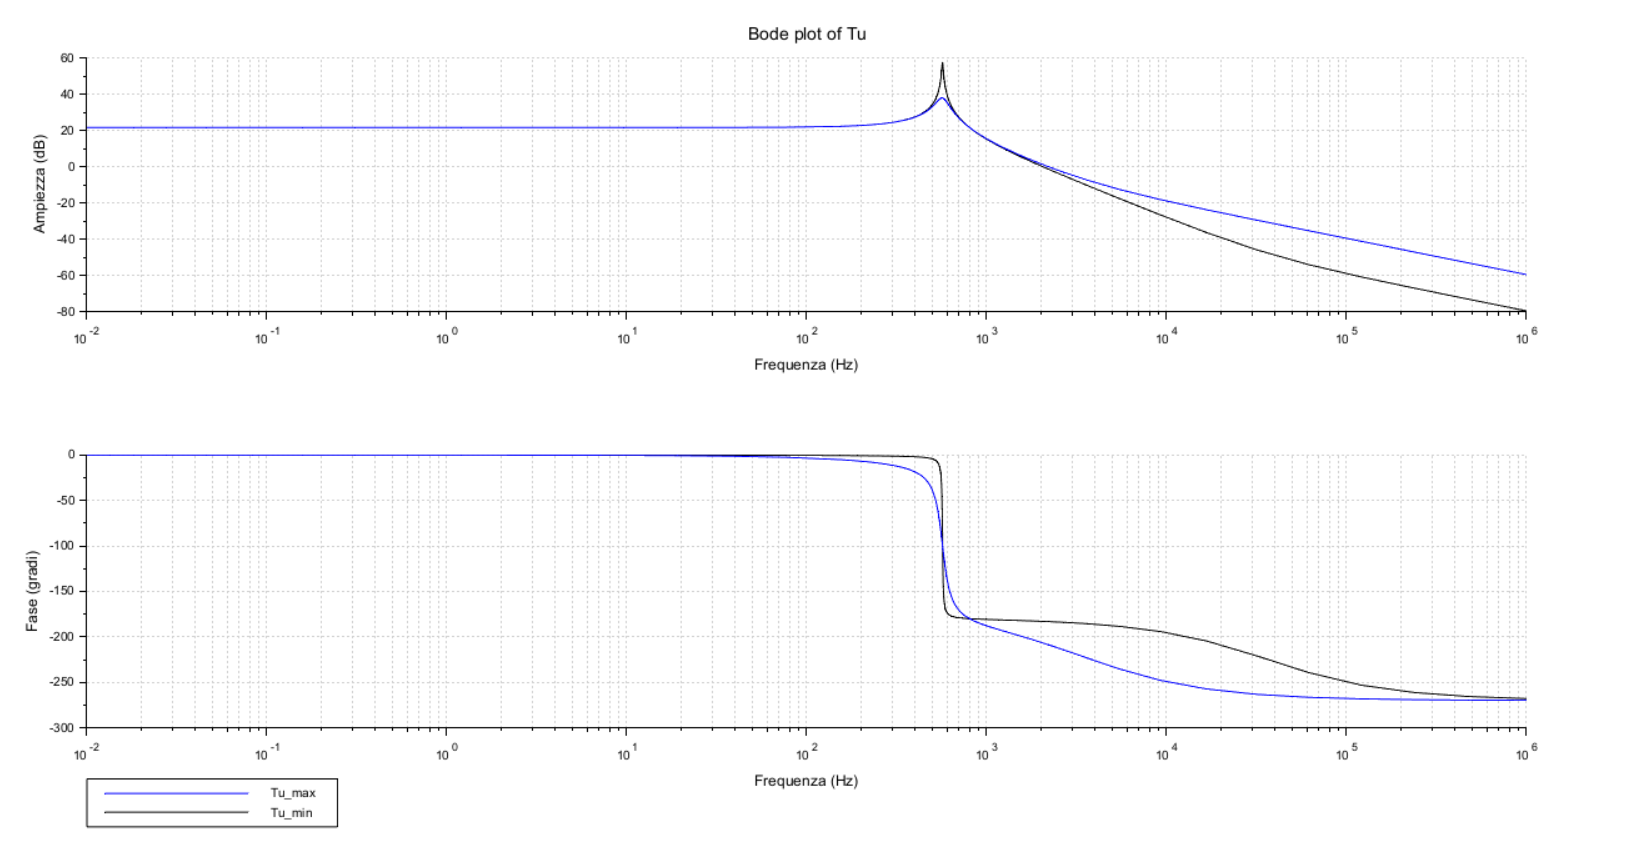
\includegraphics[width=1\textwidth]{img/bode Tu(s).png}
    \caption{Diagramma di bode della funzione di trasferimento \(T_u(s)\)}
    \label{fig:bode Tu(s)}
\end{figure}
\vspace{0.5em}

\noindent
Si nota come \(T_u(s)\) non sia stabile ad anello chiuso, infatti il margine di fase e di guadagno sono

\vspace{0.5em}
\begin{align*}
    \phi_{m_{min}} &= -28.6\text{°} \ \ \
    \phi_{m_{max}} = -2.95\text{°} \\
    M_{g_{min}} &= -21.6dB \ \ \ 
    M_{g_{max}} = -21.6dB
\end{align*}
\vspace{0.5em}

\noindent
quindi per qualunque valore della resistenza di carico compreso nel range delle specifiche, entrambi i margini sono negativi.
Per stabilizzare la risposta ad anello chiuso e rispettare la specifica di \(\epsilon_r \leq 1\%\ \) a regime si può utilizzare un controllore PI. \\
Per cercare di rispettare la specifica di \(\epsilon_r(50Hz) \leq 10 \%\ \) si cerca di portare il modulo di \(T(s)\) abbastanza in basso da avere \(\omega^*\) prima di \(\omega_o\), dove con \(\omega^*\) si intende la pulsazione per cui \(|T(\omega^*)|_{dB} = 0dB\), così da avere un margine di fase positivo e prossimo a \(90\text{°}\), ma comunque cercando di mantenere \(\omega^*\) il più in alto possibile.
Il valore massimo di \(K_T\) si ha quando il picco di \(|T(s)|\) in \(\omega_o\) tocca l'asse a \(0dB\), poichè sopra quella soglia avrei che \(T(s)\) passa più volte per \(0dB\), quindi

\vspace{0.5em}
\[
    K_T \frac{|T_u(0)|Q_{max}}{s} < 1 \implies K_T < 4.63
\]
\vspace{0.5em}

\newpage
\noindent
La frequenza di zero del controllore va piazzata dopo la pulsazione \(\omega_o\), quindi un esempio di controllore utilizzabile è il seguente

\vspace{0.5em}
\[
    G_{c_{PI}}(s) = \frac{4}{s} (1 + \frac{s}{2 \pi \cdot 6000})
\]
\vspace{0.5em}

\noindent
Calcoliamo adesso l'errore \(\epsilon_r(50Hz)\) con questo controllore per vedere se la specifica è rispettata

\vspace{0.5em}
\begin{align*}
    T(50Hz) &\simeq T_u(0) \ \ \ \ \ \ \ \ \ \ \ \ \ \
    G_{c_{PI}}(50Hz) \simeq  \left. \frac{4}{j\omega} \right|_{\omega = 2\pi \cdot 50Hz} \\
    \left| \frac{1}{1+T(j\omega)} \right| &\simeq \sqrt{\frac{\omega^2}{\omega^2 + (4 \cdot T_u(0))^2}} \implies \left| \frac{1}{1+T(j\omega)} \right|_{\omega=2\pi \cdot 50Hz} \simeq 0.78 > 0.1
\end{align*}
\vspace{0.5em}

\noindent
quindi la specifica di \(\epsilon_r(50Hz) \leq 10 \%\) non è rispettata con questo tipo di controllore. \\
Per riuscire a rispettare anche questa specifica si opta per un controllore a due zeri e tre poli di cui uno nell'origine, quindi un controllore che ha la forma seguente

\vspace{0.5em}
\[
    G_c(s) = \frac{(1+\frac{s}{\omega_{z1}})(1+\frac{s}{\omega_{z2}})}{s(1+\frac{s}{\omega_{p1}})(1+\frac{s}{\omega_{p2}})}
\]
\vspace{0.5em}

\noindent
Questa tipologia di controllore è approfondita al seguente link

\vspace{0.5em}
\noindent
Link all'analisi del compensatore scelto, fatta da Texas Instruments
\begin{center}
    \url{https://www.ti.com/lit/an/slva662/slva662.pdf?ts=1755498934755&ref_url=https%253A%252F%252Fwww.google.com%252F}
\end{center}
\vspace{0.5em}

\vspace{0.5em}
\begin{figure}[h]
    \centering
    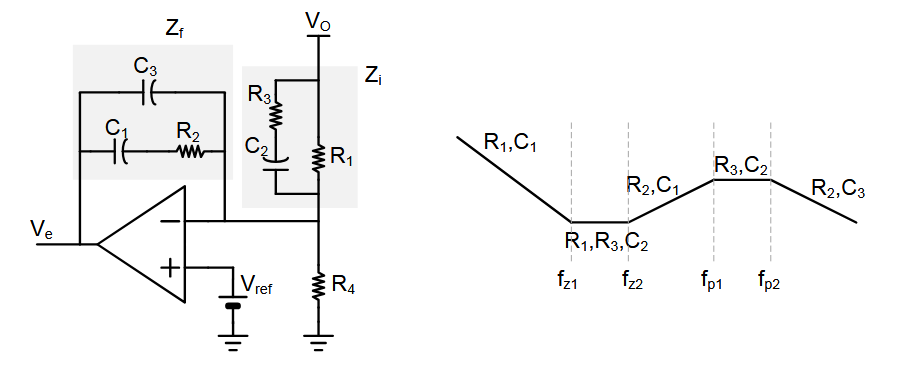
\includegraphics[width=0.6\textwidth]{img/compensatore III.png}
    \caption{Esempio di compensatore utilizzato preso dal sito di Texas Instruments}
    \label{fig:compensatore III}
\end{figure}
\vspace{0.5em}

\noindent
Per il dimensionamento del controllore scelto si parte dagli zeri della funzione di trasferimento. \\
Il primo zero serve per appiattire \(T(s)\) prima della pulsazione di risonanza \(\omega_o\) e dovrà essere tale da garantire un \(|T(50Hz)|\) sufficiente ad avere \(\epsilon_r(50Hz)<10 \%\), quindi

\vspace{0.5em}
\begin{align*}
    \left| \frac{1}{1+T(50Hz)} \right|_{dB} < -20dB \implies |1+T(50Hz)|_{dB} > 20dB
\end{align*}
\vspace{0.5em}

\noindent
visto che \(|1+T(50Hz)|_{dB} > |T(50Hz)|_{dB}\) la specifica è rispettata anche se \(|T(50Hz)|_{dB} > 20dB\), quindi 

\vspace{0.5em}
\[
    \frac{T_u(0)}{\omega_{z1}} > 10 \implies \omega_{z1} < \frac{T_u(0)}{10} \simeq 1.2 \implies f_{z1} = \frac{\omega_{z1}}{2 \pi} \simeq 0.19
\]
\vspace{0.5em}

\noindent
Per quanto riguarda il secondo zero, è quello che permette di avere un miglioramento del margine di fase alzando la fase e lasciando invariato il modulo di \(T(s)\) in corrispondenza di \(\omega^*\), quindi deve essere tale che \(|G_c(f^*)|=1\).

\noindent
Per prima cosa calcolo il valore di \(\omega^*\)

\vspace{0.5em}
\[
    \left| \frac{T_u(0)}{(1+\frac{j\omega^*}{\omega_o})^2} \right| = 1 \implies \omega^* = \omega_o\sqrt{T_u(0)-1} \simeq 11834 \frac{rad}{s} \implies f^* = \frac{\omega^*}{2 \pi} \simeq 1883 Hz
\]
\vspace{0.5em}

\noindent
una volta calcolato il valore di \(\omega^*\) devo posizonare lo zero in modo tale che \(|G_c(f^*)|=1\)

\vspace{0.5em}
\begin{align*}
    \left| G_c(50Hz) \left[ 1+\frac{j\omega^*}{\omega_{z2}} \right] \right| &= 1 \implies \frac{1}{\left | G_c(50Hz)\right | ^2} = 1 + \frac{{\omega^{*}}^{2}}{\omega_{z2}^2} \\ 
    \implies {\omega_{z2}} &= \omega^*\sqrt{\frac{1}{\frac{1}{\left| G_c(50Hz) \right|} - 1}} \simeq 17840 \frac{rad}{s} \implies f_{z2} = \frac{\omega_{z2}}{2 \pi} \simeq 2839Hz
\end{align*}
\vspace{0.5em}

\noindent
Una volta posizionati gli zeri, i poli basta piazzarli a frequenza più alta di \(\omega^*\), nel nostro caso sono stati posizionati a \(3\cdot10^5 \frac{rad}{s}\) e a \(3\cdot10^6 \frac{rad}{s}\), quindi all'incirca due decadi più in là dello zero a più alta frequenza. \\
Il controllore è stato poi simulato e i parametri calcolati sopra sono stati aggiustati in modo da migliorare il margine di fase e di guadagno della funzione di trasferimento reale (non asintotica, che è quella che è stata analizzata per dimensionare il controllore).\\
Il controllore utilizzato è il seguente

\vspace{0.5em}
\[
    G_c(s) = \frac{(1+\frac{s}{2 \pi 0.25})(1+\frac{s}{2 \pi 1000})}{s(1+\frac{s}{2 \pi 60000})(1+\frac{s}{2 \pi 600000})}
\]
\vspace{0.5em}

dalla simulazione, la funzione di trasferimento \(T(s)\) controllata è quella in \autoref{fig:bode diagrams CL} 

\vspace{0.5em}
\begin{figure}[h]
    \centering
    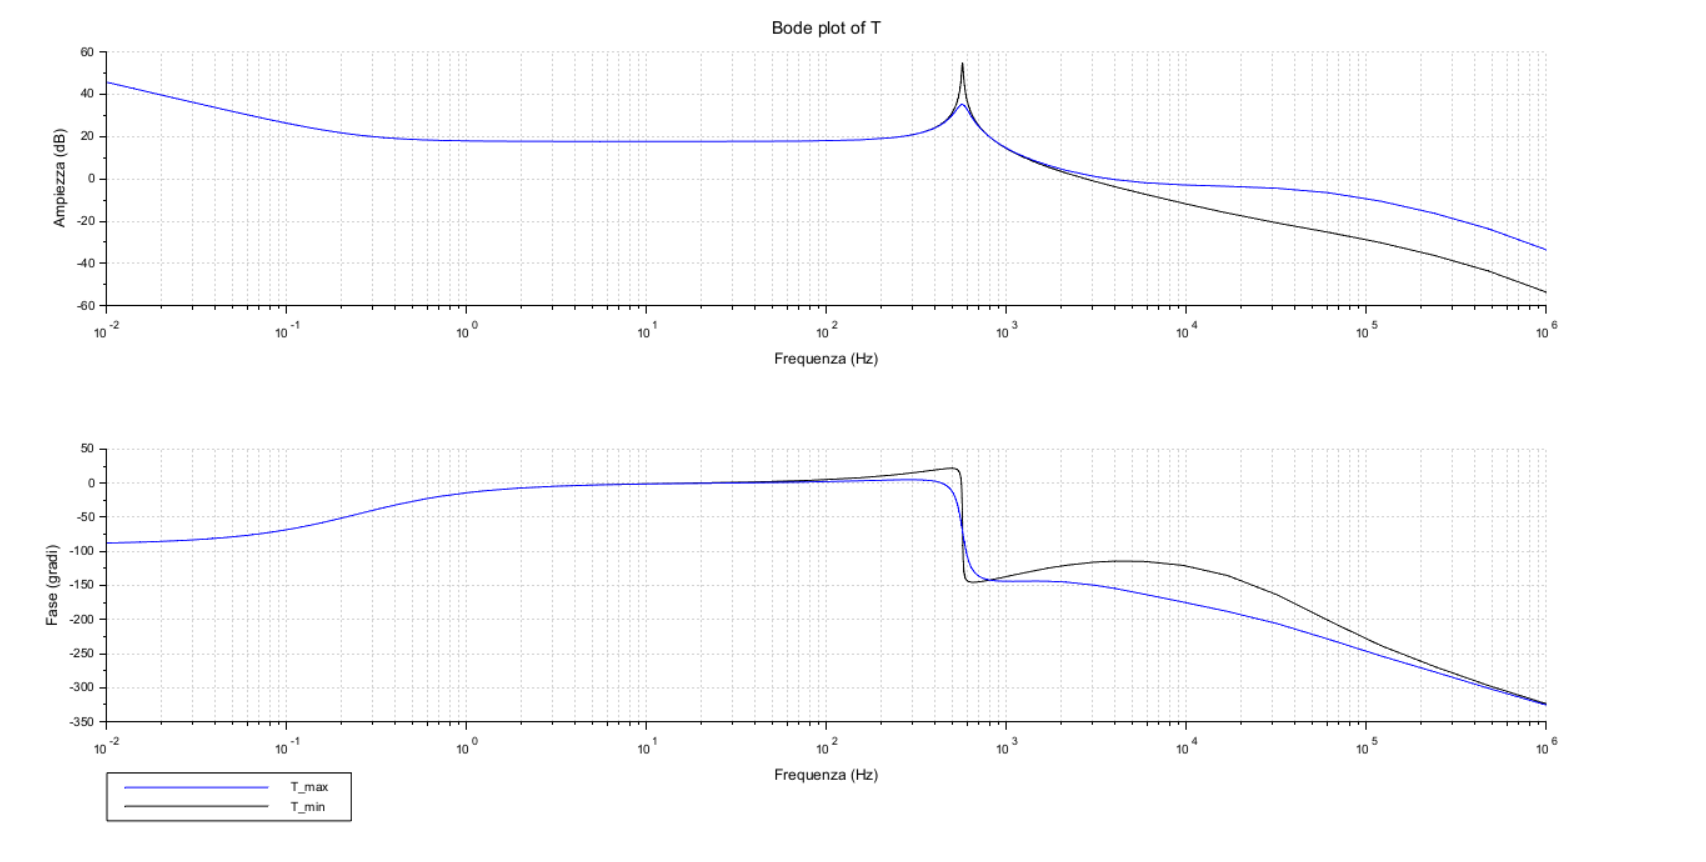
\includegraphics[width=1\textwidth]{img/bode diagrams CL.png}
    \caption{funzione di trasferimento di \(T(s)\) con il compensatore dimensionato}
    \label{fig:bode diagrams CL}
\end{figure}
\vspace{0.5em}

\newpage
\noindent
La funzione di trasferimento di \(E(s)=\frac{1}{1+T(s)}\) è quella in \autoref{fig:bode diagrams E} 

\vspace{0.5em}
\begin{figure}[h]
    \centering
    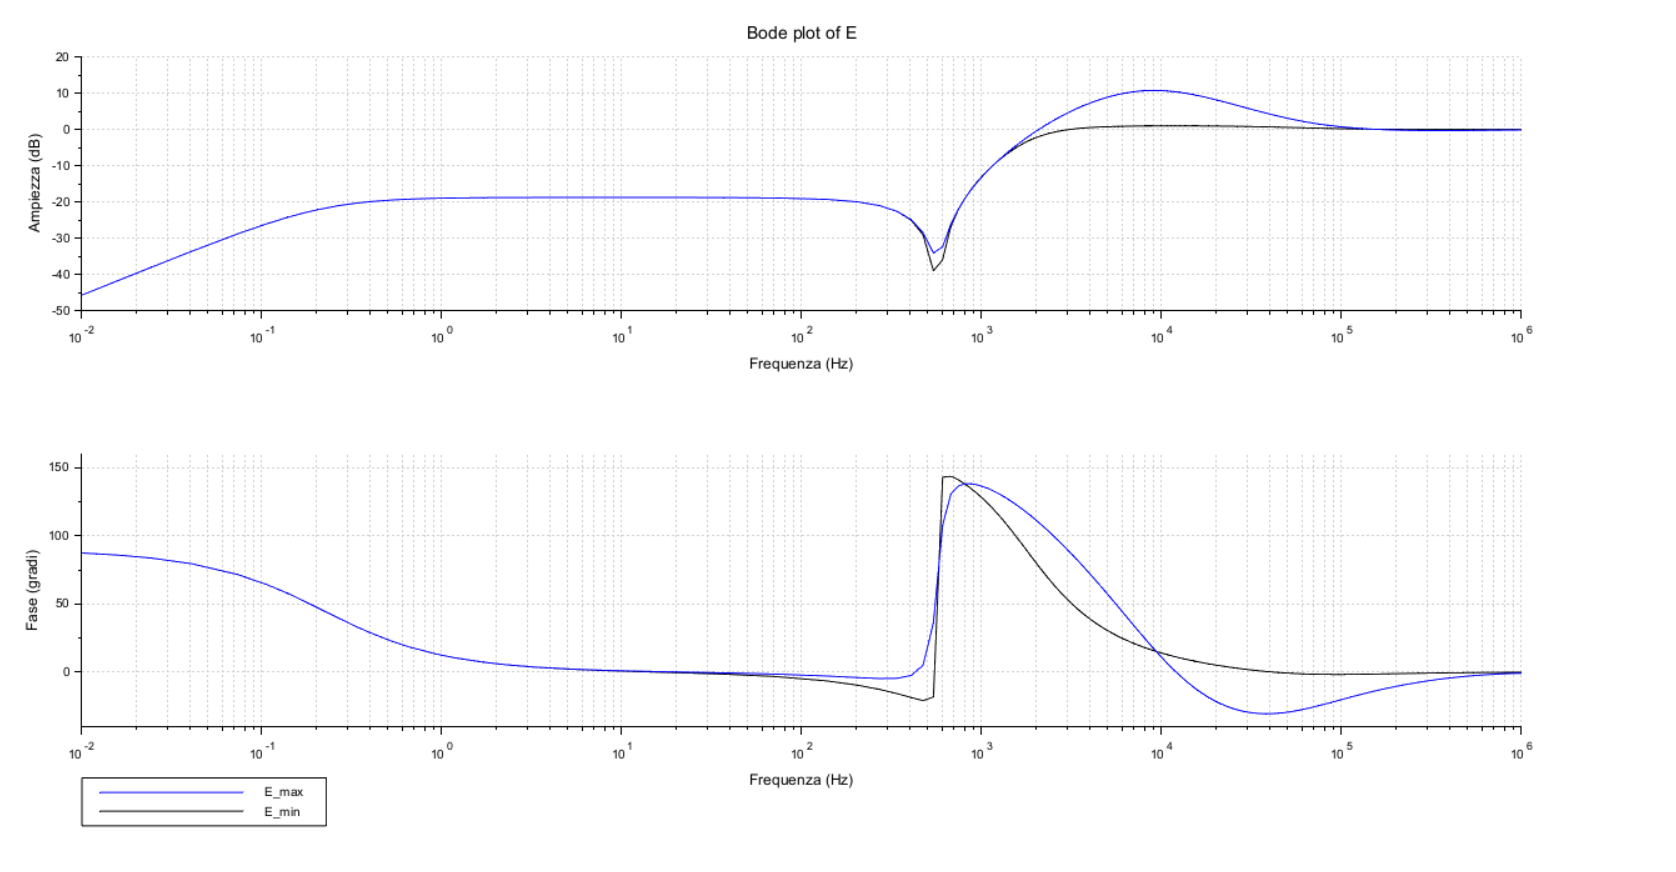
\includegraphics[width=1\textwidth]{img/bode diagrams E(s).png}
    \caption{funzione di trasferimento di \(E(s)\) con il compensatore dimensionato}
    \label{fig:bode diagrams E}
\end{figure}
\vspace{0.5em}

\noindent
La funzione di trasferimento di \(G_c(s)\) è quella in \autoref{fig:bode diagrams C} 

\vspace{0.5em}
\begin{figure}[h]
    \centering
    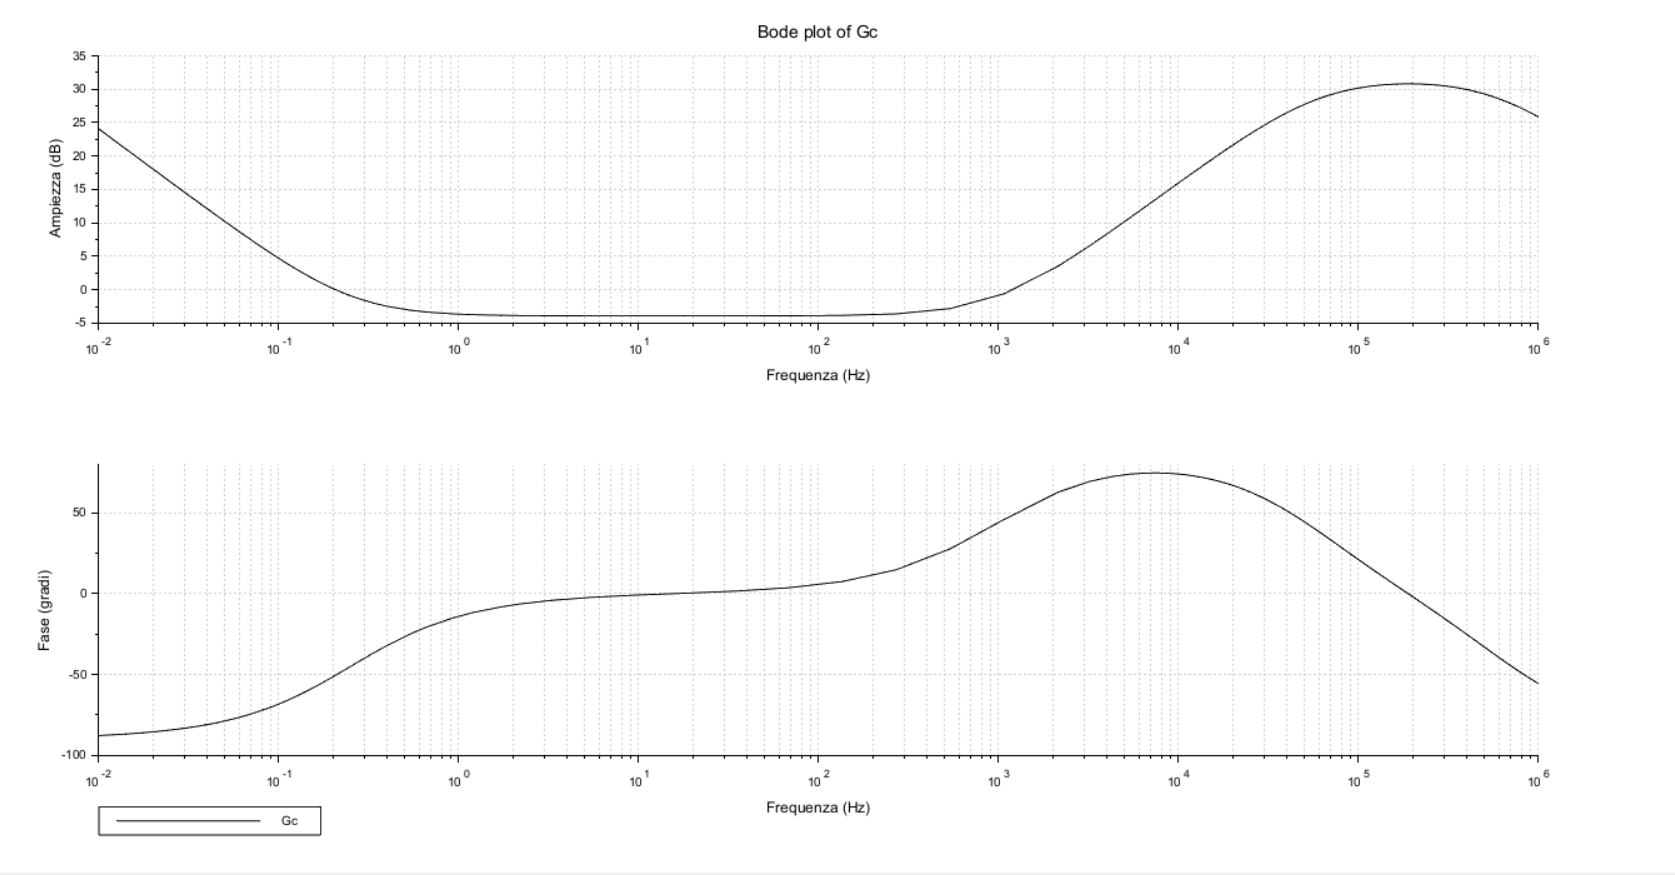
\includegraphics[width=0.98\textwidth]{img/bode diagrams C(s).png}
    \caption{funzione di trasferimento di \(G_c(s)\) dimensionato}
    \label{fig:bode diagrams C}
\end{figure}
\vspace{0.5em}

\noindent
I margini di fase e di guadagno di \(T(s)\) adesso sono 

\vspace{0.5em}
\begin{align*}
    \phi_{m_{min}} &= 26.9\text{°} \ \ \
    \phi_{m_{max}} = 63\text{°} \\
    M_{g_{min}} &= 3.2dB \ \ \ 
    M_{g_{max}} = 23.2dB
\end{align*}
\vspace{0.5em}

\noindent
quindi oltre ad essere tutti positivi (sistema retroazionato stabile per ogni condizione di carico compresa nelle specifiche) ho all'incirca \(3.2dB\) di margine di guadagno e \(26.9 \text{°}\) di margine di fase nel caso peggiore.
L'errore a regime è nullo, poichè il controllore ha un polo nell'origine, quindi rispetta la condizione \(\epsilon_r \leq 1 \%\ \) e a \(50Hz\) ho che \(|\epsilon_r(50Hz)|_{dB} \simeq -20dB \implies \epsilon_r(50Hz) \simeq 0.1\) quindi è rispettata anche la specifica di \(\epsilon_r(50Hz) \leq 10 \%\ \). \\

\newpage
\section{Simulazione circuito di feedback}
Per la simulazione, prima di tutto si verifica con LTSpice che la funzione di trasferimento \(G_{vd}(s)\) calcolata in precedenza sia giusta utilizzando il modello dinamico del convertitore \autoref{fig:modello dinamico 2}

\vspace{0.5em}
\begin{figure}[h]
    \centering
    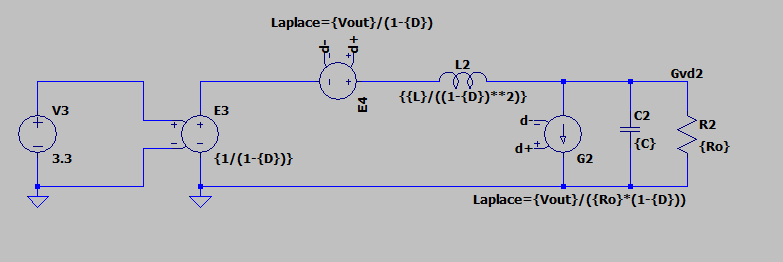
\includegraphics[width=0.7\textwidth]{img/modello dinamico 2.png}
    \caption{Modello dinamico del convertitore}
    \label{fig:modello dinamico 2}
\end{figure}
\vspace{0.5em}

\noindent
si può anche utilizzare il modello del convertitore in forma canonica \autoref{fig:modello dinamico 1}, sono equivalenti

\vspace{0.5em}
\begin{figure}[h]
    \centering
    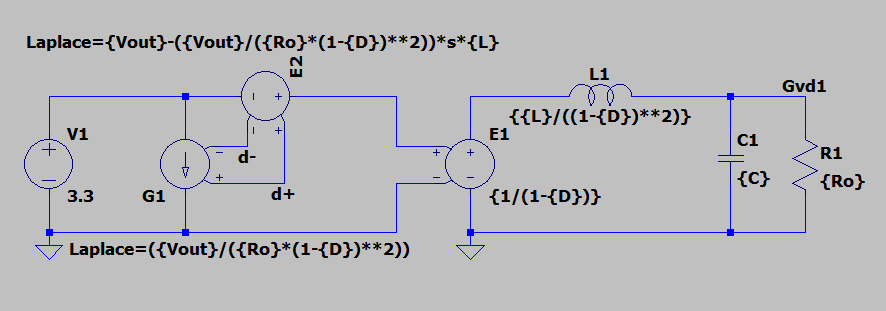
\includegraphics[width=0.7\textwidth]{img/modello dinamico 1.png}
    \caption{Modello dinamico del convertitore in forma canonica}
    \label{fig:modello dinamico 1}
\end{figure}
\vspace{0.5em}

\noindent
La funzione di trasferimento simulata è concorde con i calcoli effettuati sopra, come si nota dalla figura \autoref{fig:Gvd LTSpice}

\vspace{0.5em}
\begin{figure}[h]
    \centering
    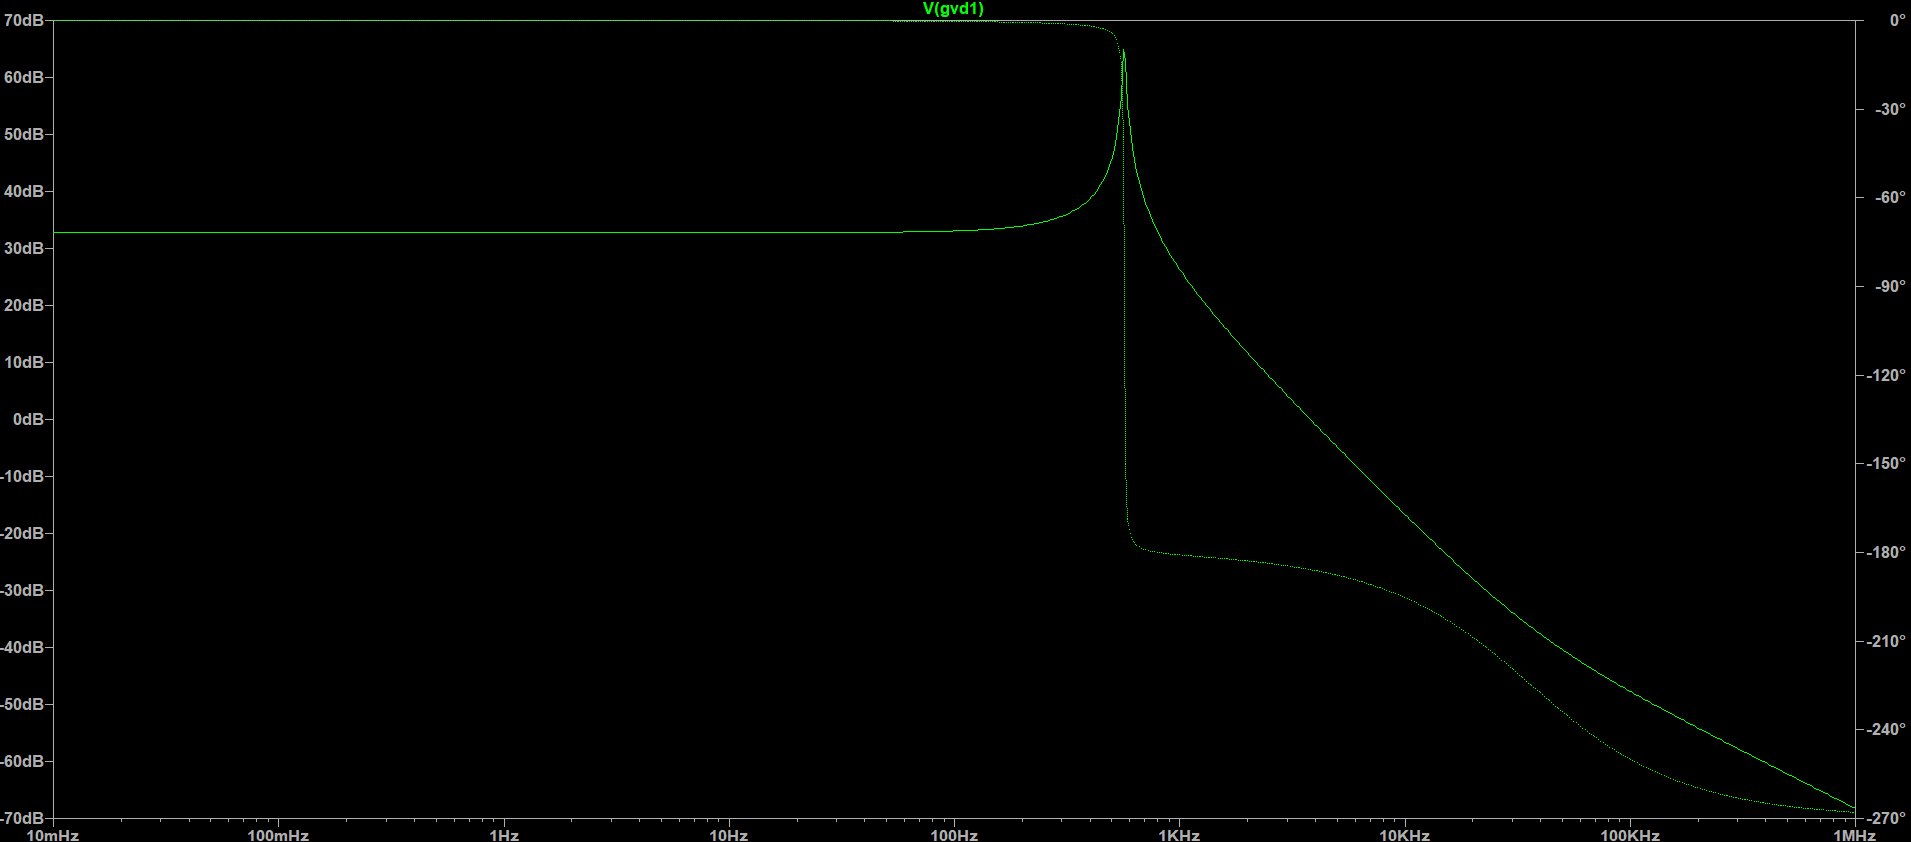
\includegraphics[width=1\textwidth]{img/Gvd LTSpice.png}
    \caption{\(G_{vd}(s)\) ottenuta con il simulatore LTSpice}
    \label{fig:Gvd LTSpice}
\end{figure}
\vspace{0.5em}

\newpage
\noindent
Adesso valutiamo la risposta al gradino del sistema non retroazionato e per fare questo usiamo Xcos (un tool di Scilab).
Il sistema simulato è il seguente \autoref{fig:XCOS modello open loop}

\vspace{0.5em}
\begin{figure}[h]
    \centering
    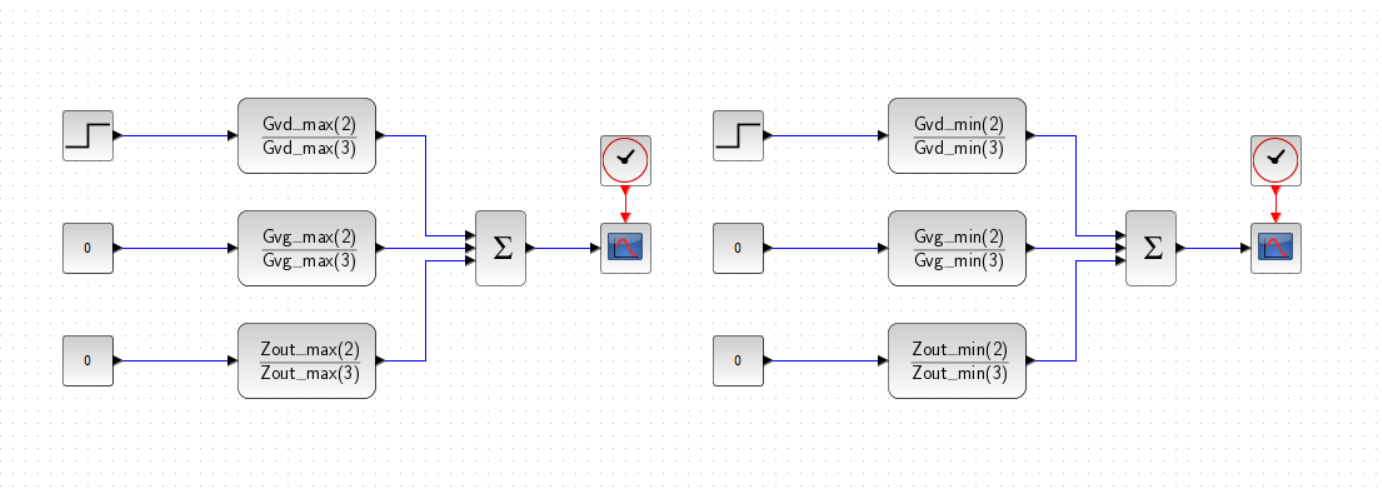
\includegraphics[width=1\textwidth]{img/XCOS modello open loop.png}
    \caption{Sistema ad anello aperto simulato su Xcos}
    \label{fig:XCOS modello open loop}
\end{figure}
\vspace{0.5em}

\noindent
Mandiamo in ingresso al blocco \(G_{vd}(s)\) una sollecitazione a gradino di ampiezza \(\frac{1}{G_{vd}(0)}\) in modo da avere una risposta che a regime si assesta ad un valore unitario, mentre mandiamo un ingresso nullo in ingresso ai blocchi \(Z_{out}(s)\) e \(G_{vg}(s)\).
Il risultato della simulazione è il seguente \autoref{fig:XCOS risposta open loop}, le risposte sono due, una ottenuta con un carico di \(R_{out}=100\Omega\) e una con un carico di \(R_{out}=1000\Omega\), quindi ottenute agli estremi di funzionamento nominale del convertitore.

\vspace{0.5em}
\begin{figure}[h]
    \centering
    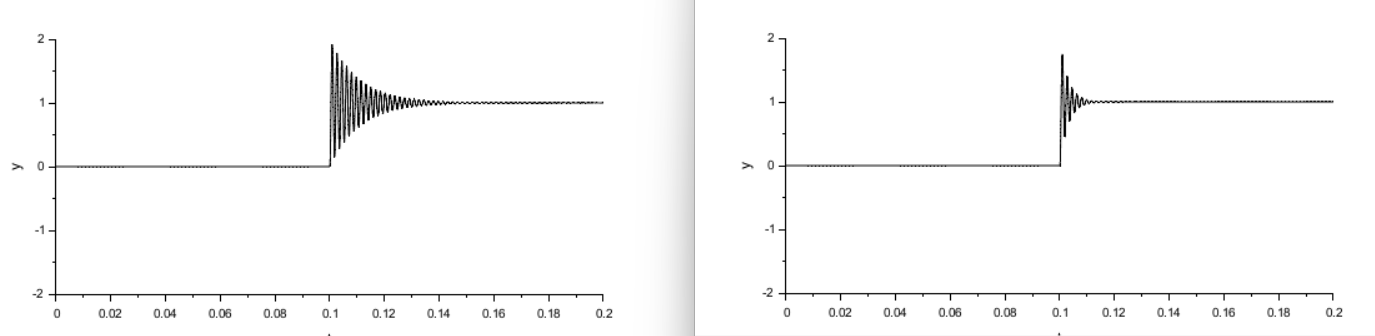
\includegraphics[width=1\textwidth]{img/XCOS risposta open loop.png}
    \caption{Risposta al gradino sistema ad anello aperto}
    \label{fig:XCOS risposta open loop}
\end{figure}
\vspace{0.5em}

\newpage
\noindent
Chiudendo il sistema in feedback con il controllore \(G_c(s)\) calcolato precedentemente la risposta cambia, quindi si simula la risposta del sistema ad un gradino da \(0V\) a \(3.3V\) della \(V_{ref}\). \\
Il modello simulato è quello in figura \autoref{fig:XCOS modello closed loop}

\vspace{0.5em}
\begin{figure}[h]
    \centering
    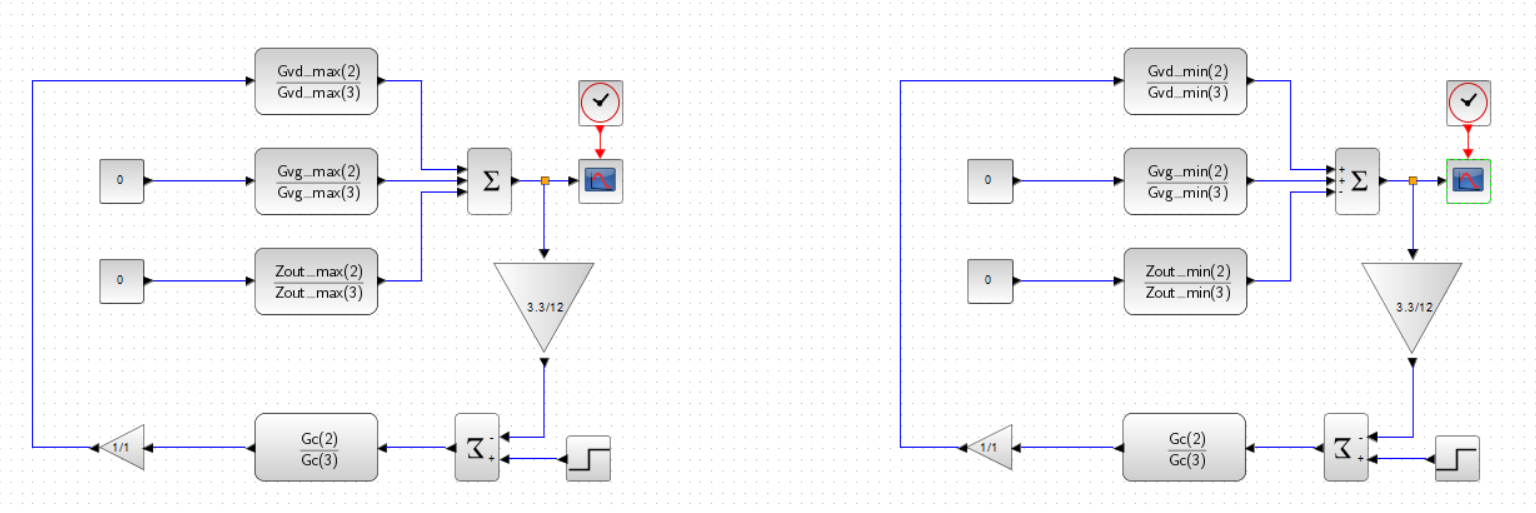
\includegraphics[width=1\textwidth]{img/XCOS modello closed loop.png}
    \caption{Sistema ad anello chiuso simulato su Xcos}
    \label{fig:XCOS modello closed loop}
\end{figure}
\vspace{0.5em}

\noindent
La risposta al gradino si ottiene, come per il caso ad anello aperto, mettendo un ingresso nullo ai blocchi \(G_{vg}(s)\) e \(Z_{out}(s)\) e collegando in retroazione il compensatore al blocco \(G_{vd}(s)\). \\
La risposta ad anello chiuso è quella in figura \autoref{fig:XCOS risposta closed loop}, ottenuta anche qui per un carico \(R_{out} = 100 \Omega\) e \(R_{out} = 1000 \Omega\).

\vspace{0.5em}
\begin{figure}[h]
    \centering
    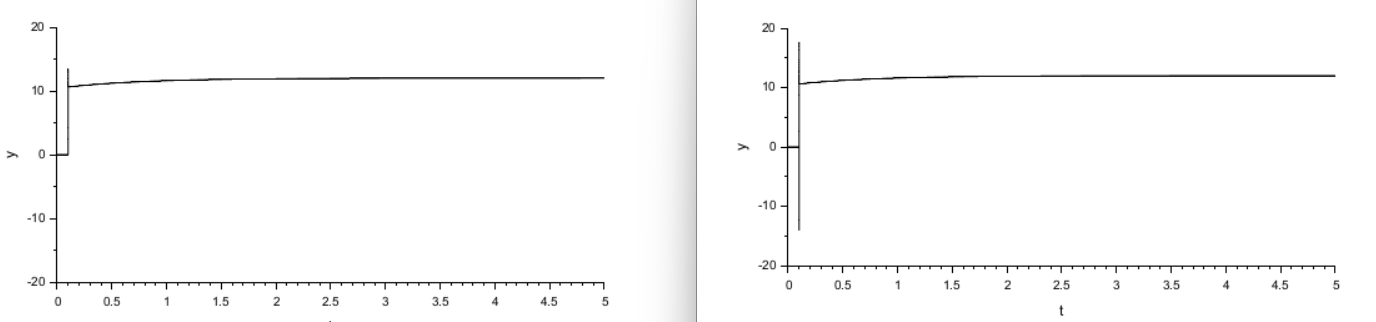
\includegraphics[width=1\textwidth]{img/XCOS risposta closed loop.png}
    \caption{Risposta al gradino sistema ad anello chiuso}
    \label{fig:XCOS risposta closed loop}
\end{figure}
\vspace{0.5em}

\newpage
\noindent
L'ultima simulazione da fare è quella su LTSpice del sistema ad anello chiuso. \\
Per prima cosa si verifica che la funzione di trasferimento del compensatore, sia concorde con la \(G_c(s)\) calcolata analiticamente.

\vspace{0.5em}
\begin{figure}[h]
    \centering
    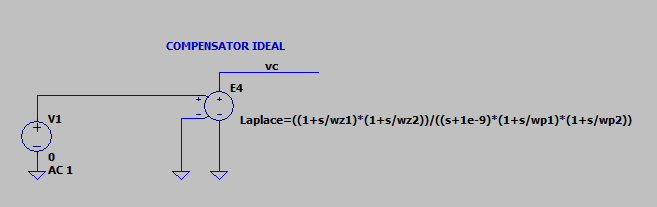
\includegraphics[width=1\textwidth]{img/Laplace compensatore.png}
    \caption{Blocco compensatore ideale LTSpice}
    \label{fig:Laplace compensatore}
\end{figure}
\vspace{0.5em}

\vspace{0.5em}
\begin{figure}[h]
    \centering
    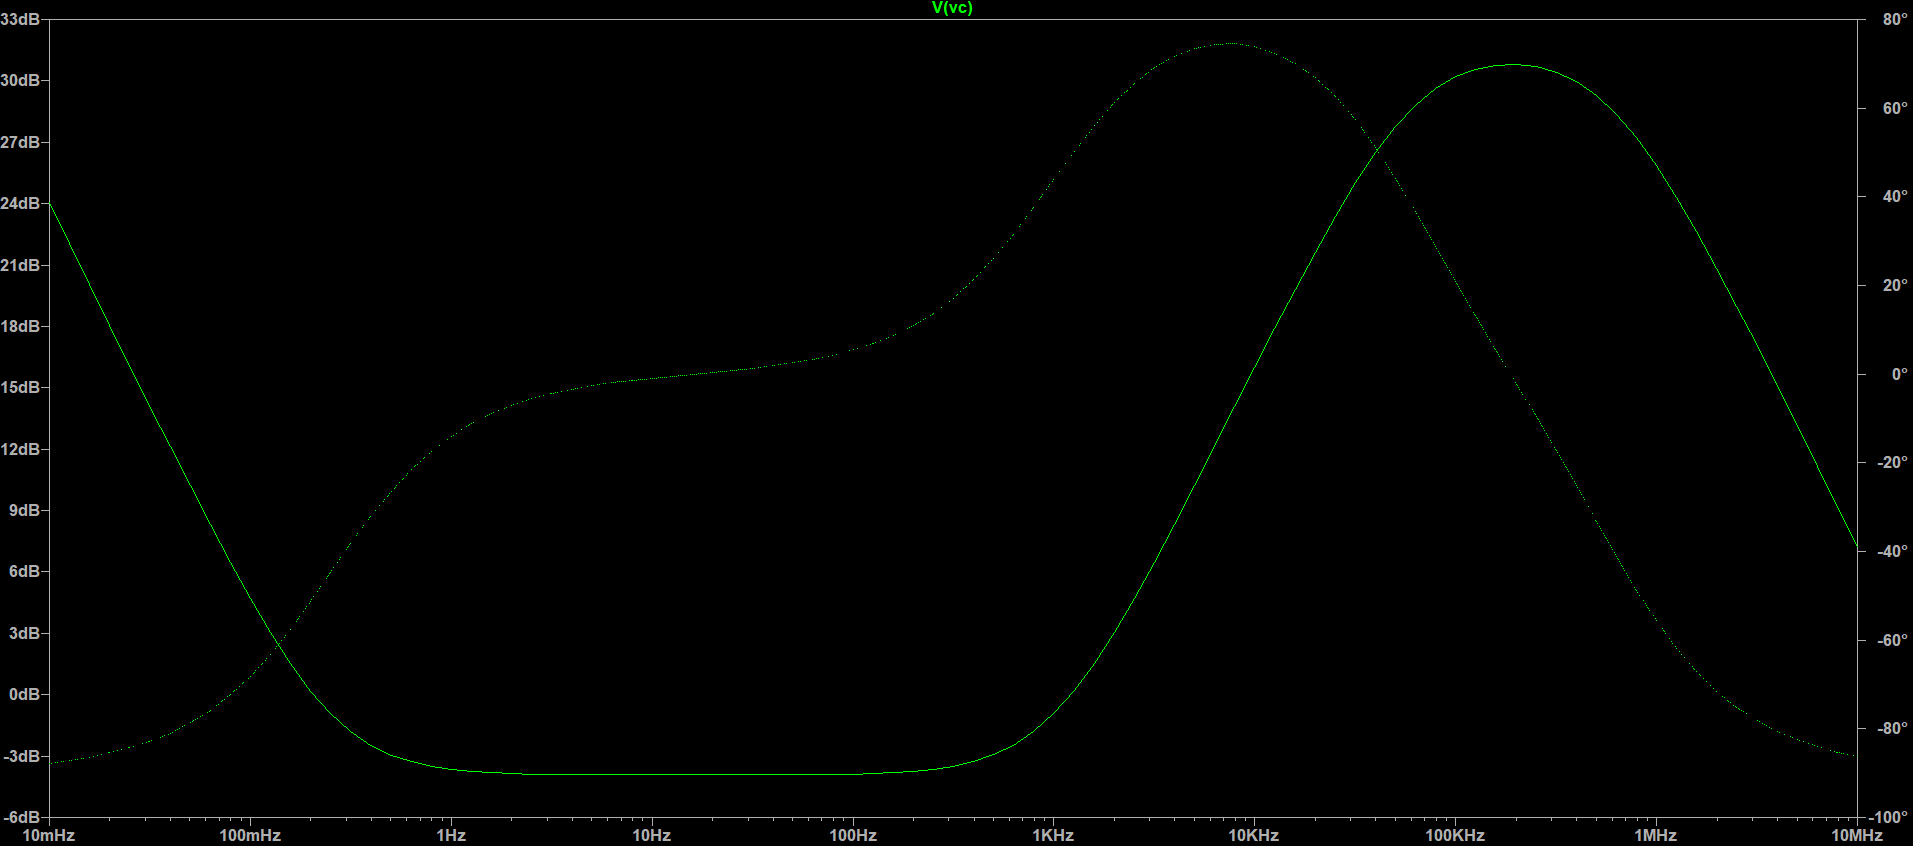
\includegraphics[width=1\textwidth]{img/Grafico Laplace compensatore.png}
    \caption{funzione di trasferimento del blocco compensatore ideale LTSpice}
    \label{fig:Grafico Laplace compensatore}
\end{figure}
\vspace{0.5em}

\newpage
\noindent
Dopo aver verificato che il compensatore abbia la funzione di trasferimento calcolata analiticamente, si simula tutto il sistema retroazionato con il controllore scelto \(G_c(s)\). \\
Il circuito simulato è quello in figura \autoref{fig:simulazione anello chiuso}

\vspace{0.5em}
\begin{figure}[h]
    \centering
    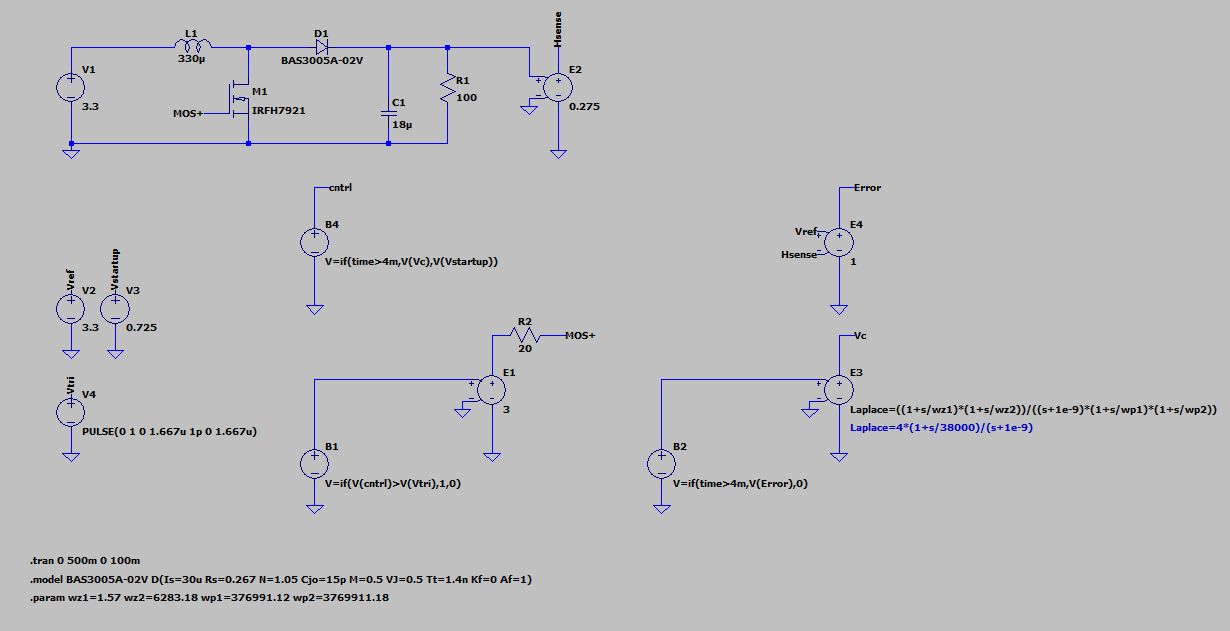
\includegraphics[width=1\textwidth]{img/simulazione anello chiuso.png}
    \caption{Circuito utilizzato su LTSpice per effettuare la simulazione del sistema retroazionato}
    \label{fig:simulazione anello chiuso}
\end{figure}
\vspace{0.5em}

\noindent
Dalla simulazione risulta che la tensione in uscita del convertitore tende alla tensione \(V_{out}\) e la tensione \(V_{err}\) tende a zero a regime.
Con un carico di \(R_o = 100 \Omega\) si arriva a regime dopo circa \(1s\).

\vspace{0.5em}
\begin{figure}[h]
    \centering
    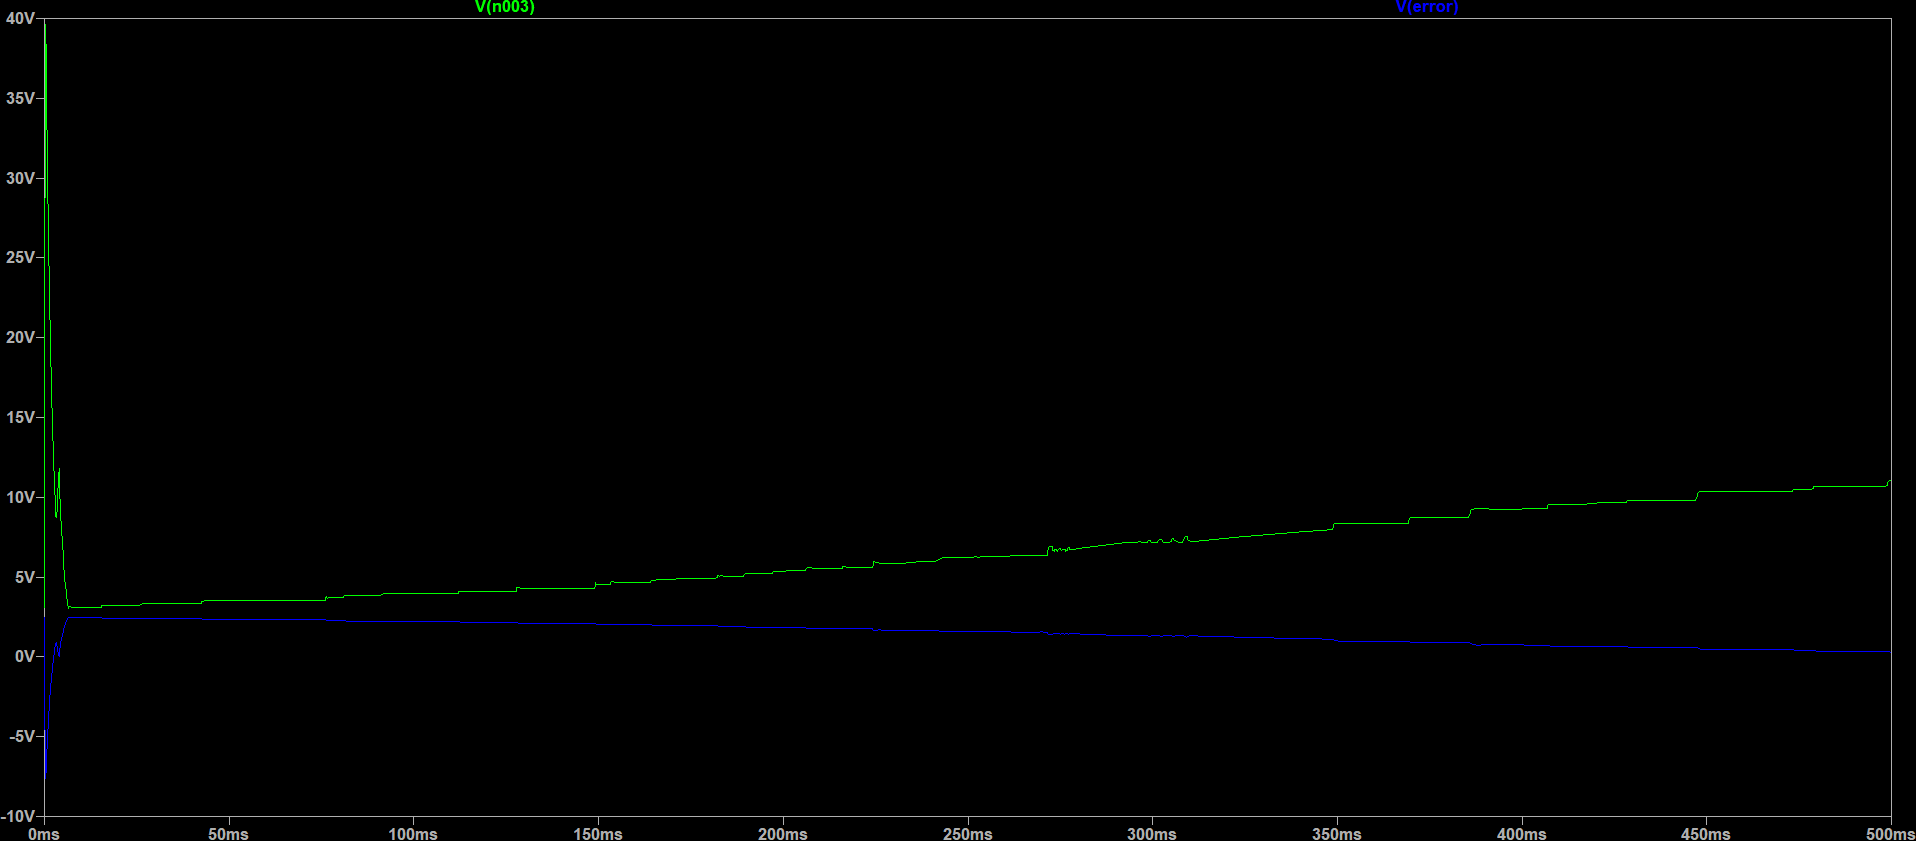
\includegraphics[width=1\textwidth]{img/simulazione anello chiuso LTSpice.png}
    \caption{Tensione \(V_{out}\) (onda verde) e tensione \(V_{err}\) (onda blu)}
    \label{fig:simulazione anello chiuso LTSpice}
\end{figure}
\vspace{0.5em}

\end{document}